\documentclass{book}
\usepackage[utf8]{inputenc}
\usepackage[ngerman]{babel}
\usepackage{enumerate}
\usepackage{amsfonts}
\usepackage[T1]{fontenc}
\usepackage{graphicx}
\usepackage{tabularx}
\usepackage{verbatim}
\usepackage[font=small,labelfont=bf]{caption}
\usepackage[absolute]{textpos}
\usepackage{pdfpages}
\usepackage{algorithm}
\usepackage{algorithmic}
\usepackage{hyperref}

\newcommand{\bibiserv}{\textit{BiBiServ2}}

\newcommand{\bibiservsearch}{\textit{BiBiServSearch}}

%figure standard befehl für Graphen
\newcommand{\graph}[3]{
\begin{figure}
\centering
\includegraphics[scale=0.85]{#1}
\caption{#3}
\label{#2}
\end{figure}
}

\begin{document}

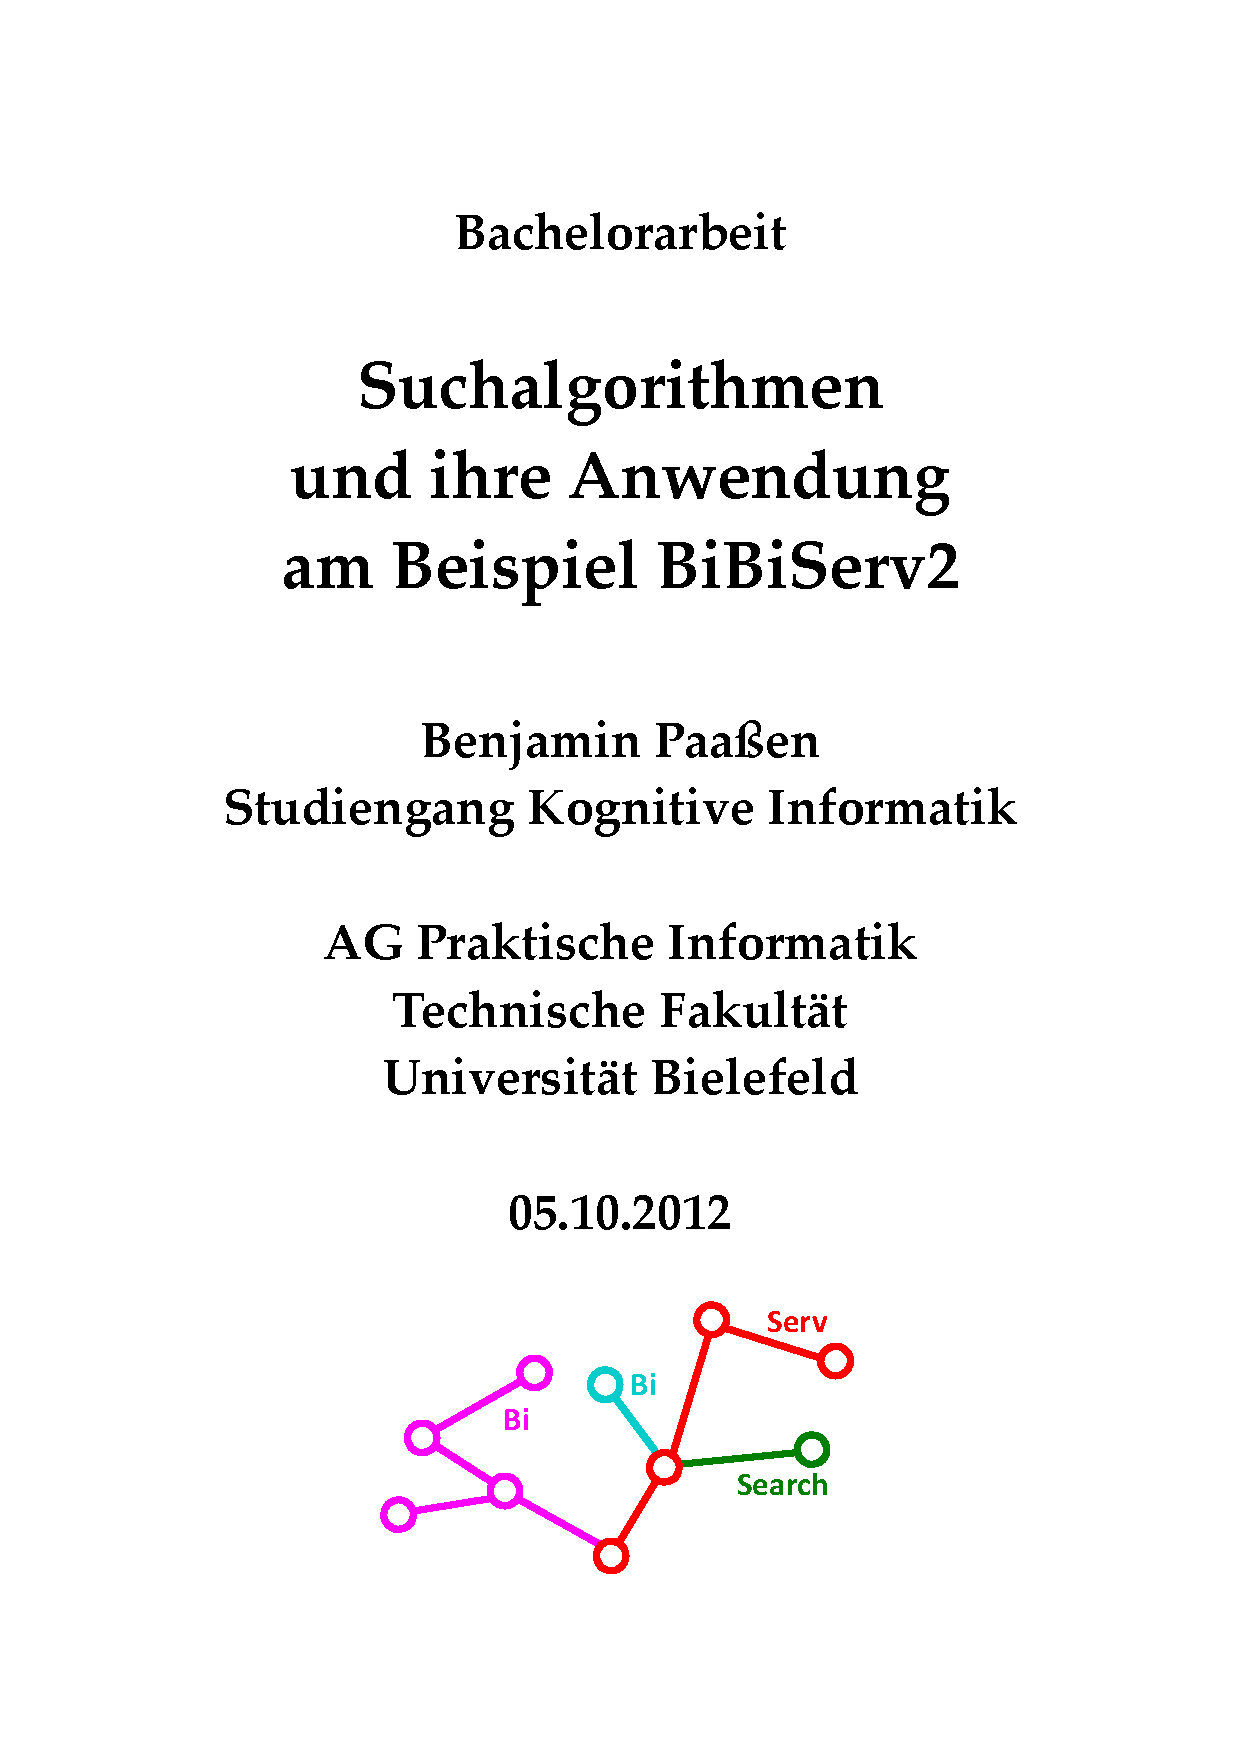
\includepdf{resources/titlepage.pdf}

\paragraph{Bachlorarbeit} von Benjamin Paaßen, Student der Kognitiven Informatik an der Technischen Fakultät der Universität Bielefeld.

\paragraph{Abgabefrist:} 05.10.2012

\paragraph{Programm:} Diese Arbeit betrifft das Programm \textit{BiBiServSearch}, verfügbar als Java\texttrademark-Paket auf dem CeBiTec-Server der Universität Bielefeld (\url{http://bibiserv.cebitec.uni-bielefeld.de/ivy-rep/de.unibi.cebitec.bibiserv/bibiservsearch/} [Stand 17.09.2012]).
\paragraph{} Der Programmcode ist im Mercurial\texttrademark-System des CeBiTec unter \url{ssh://hg@hg.cebitec.uni-bielefeld.de/bibiadm/bibiserv2/main/bibiservsearch} einsehbar (Stand 17.09.2012).

\paragraph{Gutachter:}

\begin{itemize}
 \item[] Prof. Dr. Robert Giegerich
 \item[] Dipl. Inf. Jan Krüger
\end{itemize}

\tableofcontents

\chapter{Einleitung}

\paragraph{} Diese Arbeit erläutert die Implementierung einer Seitensuche für die Homepage des \textit{Bielefeld Bioinformatics Service} mit dem Titel \textit{BiBiServSearch}. Eine Seitensuche gehört mittlerweile zu den üblichen Funktionen, die eine Homepage bereitstellen muss und Nutzende haben Erwartungen an Funktionsumfang und Leistungsfähigkeit einer solchen Suche. Vorgestellt wird der Versuch, diesen vielfältigen Anforderungen gerecht zu werden und dabei trotzdem kompatibel mit dem System des \textit{Bielefeld Bioinformatics Service} zu bleiben.
\paragraph{} Im folgenden wird das genaue Ziel und der Kontext der Arbeit vorgestellt. In Kapitel \ref{methoden} sind die theoretischen Grundlagen der Implementierung und in Kapitel \ref{implementierung} die Implementierung selbst beschrieben. Schließlich folgt die Analyse der Ergebnisse der Arbeit in Kapitel \ref{fazit}.

\section{Zielstellung}

\paragraph{} Zur Beschreibung des Problems dieser Arbeit sind zuerst einige Begriffe zu definieren, deren Zusammenhänge auch in einem UML-Domänenmodell im Anhang visualisiert sind (siehe \ref{uml-domain}):
\begin{itemize}
 \item Der \textbf{Suchraum} $\delta$ ist eine Menge von Dokumenten.
 \item Ein \textbf{Dokument} $d$ ist hier lediglich eine geordnete Liste von Vorkommen.
 \item Ein \textbf{Vorkommen} $v$ ist ein Vorkommen eines Wortes (z.B. hat das Wort \textbf{das} in dem Dokument "`Das Schaf sieht das Haus."' zwei Vorkommen).
 \item Ein \textbf{Suchmuster} $p$ ist eine Funktion von Worten in Wahrheitswerte.
 \item Ein \textbf{Match} $m$ für ein Suchmuster $p$ ist ein Wort, für das gilt: $p(w)$ ist wahr.
\end{itemize}

\paragraph{} Dementsprechend lassen sich zwei formale Aufgaben identifizieren:
\begin{enumerate}
 \item Für einen gegebenen Suchraum $\delta$ und ein Suchmuster $p$ alle Vorkommen $v$ zu finden, für die gilt: Das Wort von $v$ ist ein Match für $p$ (\textbf{Suchproblem}).
 \item Für die Ergebnismenge von Vorkommen eine sortierte Liste von Dokumenten erstellen, die wenigstens ein Ergebnisvorkommen enthalten, so dass \textit{das am meisten dem Suchmuster entsprechende Dokument} zuerst genannt ist (\textbf{Sortier- bzw. Scoringproblem}).
\end{enumerate}
 
\paragraph{} Diese sortierte Ergebnisliste ist das, was Nutzenden am Ende eines Suchvorgangs zurückgegeben wird (siehe auch Abbildung \ref{fig-matches-screenshot}). Die Hauptschwierigkeit des Sortierproblems ist dabei nicht, die eigentliche Sortierung der Dokumente vorzunehmen, sondern eine eindeutige Relation zu definieren, nach der die Dokumente sortierbar sind.

\begin{figure}
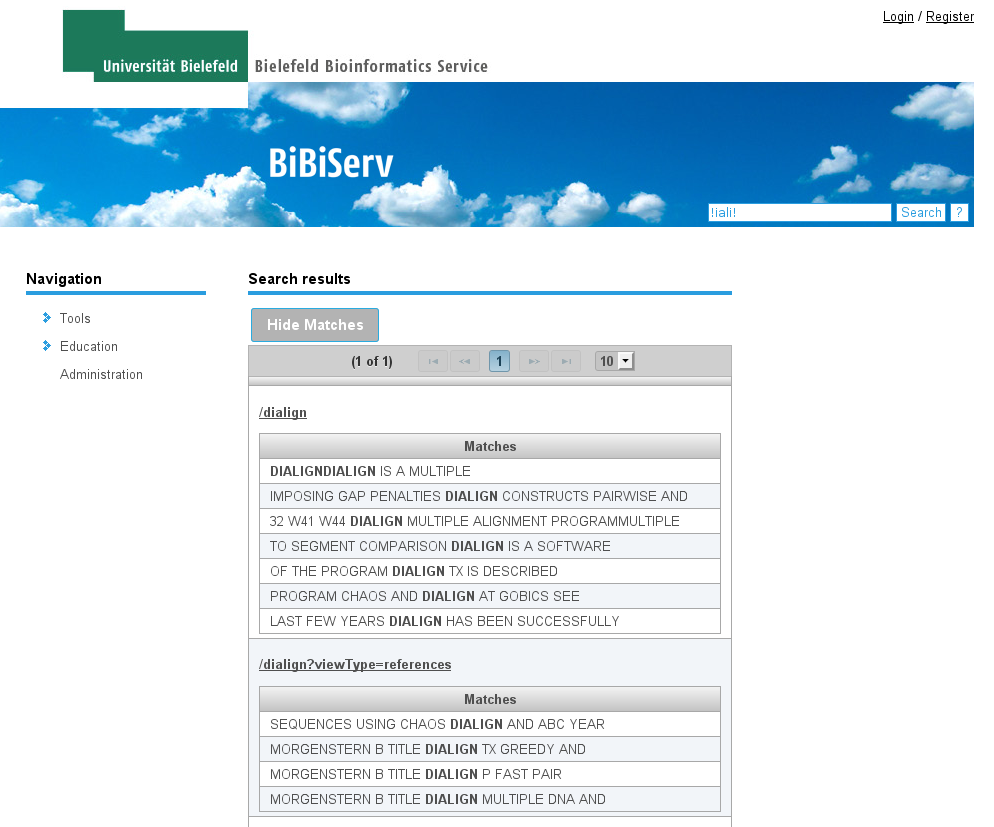
\includegraphics[scale=0.35]{resources/matches_screenshot.png}
\caption{Die Ergebnisseite der Seitensuche für den BiBiServ2. Dargestellt wird eine Liste von Links zu Dokumenten, die Vorkommen von Matches für das Suchmuster enthalten. Die Vorkommen sowie deren benachbarte Worte werden ebenfalls angezeigt.}
\label{fig-matches-screenshot}
\end{figure}

\section{BiBiServ2}

\paragraph{} Der \textit{Bielefeld Bioinformatics Service} ist eine Sammlung bioinformatischer Programme (Tools), die Nutzende aus aller Welt mittels eines Webinterface nutzen können. Der Inhalt des entsprechenden Servers \textit{BiBiServ2} besteht hauptsächlich aus diesen Webinterfaces und zusätzlichen Seiten zu den einzelnen Tools. Diese Seiten werden jedoch nicht händisch erstellt sondern dynamisch aus XML-Beschreibungen der Tools generiert(siehe auch \cite{hagemeier}, S. 5 und S. 29 f.). Dadurch wird die übliche Vorgehensweise, die Menge der HTML-Seiten als Suchraum zu definieren, wenig sinnvoll. Vielmehr besteht der Suchraum aus den Tool-Beschreibungen selbst und den durch die Beschreibungen definierten Resourcen, die auf der Homepage zur Verfügung gestellt werden. Eine Suche auf diesem ungewöhnlichen Suchraum zu ermöglichen ist die hauptsächliche Motivation dieser Arbeit.

\section{Anforderungen}
\label{anforderungen}

\paragraph{} Als Ziel der Implementierung der Suche gilt es, eine Reihe von Anforderungen zu erfüllen. Diese Anforderungen an \textit{BiBiServSearch} lassen sich in verschiedene Kategorien einteilen:

\subsection{Kompatibilität mit dem BiBiServ2}
\label{intro-compatibility}

\paragraph{} Vornehmlich ist es wichtig, dass \textit{BiBiServSearch} im Rahmen des \textit{BiBiServ2} lauffähig ist. Das bedeutet vor allem:
\begin{itemize}
 \item \textit{BiBiServSearch} muss in Java\texttrademark geschrieben sein, um als Teil des bestehenden Client-Server-Systems zu funktionieren und nahtlos in den Ablauf zum Hoch- und Herunterfahren des Servers eingefügt werden zu können.
 \item Das Programm muss XML und alle Dateiformate bearbeiten können, die als Text-Ressourcen von Tools auf dem \textit{BiBiServ2} in Frage kommen (PDF und Reintext).
 \item Die Anwendung muss in der Lage sein, mit einem dynamischen Suchraum umzugehen: Im Rahmen administrativer Zugriffe können Tools auf den Server geladen und wieder entfernt werden. Die Tools und ihre Ressourcen müssen zur Laufzeit auch in den Suchraum eingefügt bzw. daraus gelöscht werden.
\end{itemize}

\subsection{Bedienbarkeit}

\paragraph{} Zur Bedienbarkeit einer Suche tragen vor allem folgende Aspekte bei:
\begin{itemize}
 \item Nutzenden muss eine einfache und verständliche Syntax zum Ausdruck ihrer jeweiligen Suchmuster zur Verfügung gestellt werden. Dabei gilt es, möglichst nicht von den bereits üblichen Standards abzuweichen.
 \item Diese Syntax muss durch eine Hilfeseite erklärt werden.
 \item Die Ergebnisse einer Suche müssen für Nutzende nachvollziehbar sortiert werden: Das erste angezeigte Suchergebnis sollte auch dasjenige sein, dass die/der Nutzende am ehesten \textit{gemeint} hat.
 \item Die Suche sollte fehlertolerant funktionieren: Selbst wenn Nutzende sich vertippen, sollten diejenigen Suchergebnisse zurückgegeben werden, die wahrscheinlich gemeint waren.
\end{itemize}

\subsection{Funktionsumfang}
\label{anforderungen-features}

\paragraph{} In der Regel erwarten Nutzende von einer Seitensuche mehr als die Möglichkeit, einfach nur nach bestimmten Worten suchen zu können und Dokumente als Ergebnis zu erhalten, die genau dieses Wort enthalten. Vielmehr ist das Ziel, folgende Funktionen zu bieten\footnote{Hier wird um der Beispiele willen die fertige Syntax für Suchausdrücke bereits vorweggenommen. Die Syntax ist im Detail in Abschnitt \ref{algo-pattern-language} dokumentiert.}:

\paragraph{}

\begin{tabularx}{\textwidth}{llX}
\hline
\textbf{Suchmodus} & \textbf{Beispielmuster} & \textbf{Beschreibung} \\ [0.1cm]
\hline
Exakte Suche & \texttt{"holder Knabe"} & Suche nach denjenigen Dokumenten, die die Worte "`holder"' und "`Knabe"' in genau dieser Reihenfolge enthalten \\ [0.1cm]
\hline
Teilwortsuche & \texttt{!hold!} & Suche nach allen Dokumenten, die Worte enthalten, für die "`hold"' ein Teilwort ist (z.B. "`Wacholderbeere"') \\ [0.1cm]
\hline
Reguläre Ausdrücke & \texttt{![hg]old!} & Teilwortsuche nach den Worten "`hold"' \underline{und} "`Gold"' (dieses Beispiel erschöpft die Möglichkeiten regulärer Ausdrücke freilich nicht. Mehr darüber ist im Abschnitt \ref{algo-regex} zu lesen.)  \\ [0.1cm]
\hline
Inexakte Suche & \texttt{hold} & Suche nach (Teil-)worten, die dem Wort "`hold"' \textit{hinreichend ähnlich} sind. Dabei meint "`hinreichend ähnlich"' Worte, die Nutzende vielleicht eigentlich meinten, bei denen sie sich aber vertippt haben. Beispielsweise könnte bei der Suchanfrage \texttt{hold} auch "`Gold"' gemeint sein. \\ [0.1cm]
\hline
\end{tabularx}

\paragraph{} Außerdem sollte eine Veränderung des Suchraums durch administrative Anfragen nicht mit Suchanfragen von Nutzenden kollidieren. Hier sind Synchronisationsmechanismen geboten.

\subsection{Effizienzanforderungen}

\paragraph{} In Sachen Effizienz geht es sowohl um Laufzeit- als auch um Speichereffizienz. Bei der Laufzeit haben schnelle Antwortzeiten auf Suchanfragen von Nutzenden die höchste Priorität. Selbst bei schwierigen Suchmustern sollte eine Antwortzeit von maximal 3 Sekunden nicht überschritten werden. Nachrangig ist die Laufzeit bei der Bearbeitung administrativer Anfragen.
\paragraph{} Wesentlich bleibt aber die Speichereffizienz: Eine schnelle Bearbeitung von Suchanfragen erfordert die Repräsentation des Suchraums im Arbeitsspeicher. Da die Bearbeitung von Suchanfragen nicht im eigentlichen Rechengrid des \textit{BiBiServ2} stattfindet, sondern vom Server selbst übernommen wird, steht nur begrenzter Arbeitsspeicher zur Verfügung. Also ist hier eine möglichst speichereffiziente Lösung zu suchen.


\chapter{Methoden und Konzepte}
\label{methoden}

\paragraph{} Um die verschiedenen genannten Anforderungen zu erfüllen, finden sich in der Literatur eine ganze Reihe von Techniken. Es würde den Rahmen dieser Arbeit sprengen, all diese Techniken vorzustellen. Um den Umfang einzuschränken gelten daher für die weitere Betrachtung folgende Einschränkungen:
\begin{enumerate}
\item Als ideale Lösung einer exakten Suche werden hier Hashing-Techniken angesehen, weil Sie das Auffinden von Suchmustern im Suchraum (nach Vorverarbeitung) in konstanter Zeit ermöglichen (siehe \cite{knuth}, S. 538).
\item Für das Problem der Teilwortsuche gelten Suffixbäume als ideale Lösung, die für ein Suchmuster der Länge $m$ und eine Anzahl von Ergebnisvorkommen $k$ das Suchproblem in $\mathcal{O}(m + k)$, also ebenfalls unabhängig von der Größe des Suchraums, lösen können (siehe \cite{gusfield}, S. 122).
\end{enumerate}
\paragraph{} Die Nutzung von Hashing und Suffixbäumen gilt also im Folgenden als gesetzt. Die weitere Auswahl von Algorithmen und Konzepten ist in den kommenden Abschnitten erläutert. Das fertige Architekturkonzept ist in Abbildung \ref{uml-architecture} im Anhang skizziert.

\section{Indizierung und Hashing}
\label{meth-hashing}

\paragraph{} Da die Benutzung von Java\texttrademark harte Voraussetzung ist (siehe \ref{intro-compatibility}) liegt die Nutzung der Hashing-Technik nahe, die die Sprache selbst bereit stellt. Java\texttrademark\\ implementiert Hashing in der Klasse \texttt{HashMap} mit Listen zur Kollisionsbehandlung und automatischem re-hashing: Bei doppelten Hashcodes werden Elemente in Eimer für den gleichen Hashcode abgelegt. Die Suchzeit vergrößert sich dabei unter Umständen leicht. Die Eimer können allerdings nicht beliebig voll werden: Ab einer Füllung der \texttt{Map} von 75\% erhöht Java\texttrademark automatisch die Größe der Tabelle und alle Einträge werden neu gehasht (siehe auch \cite{javaHashMap}). Das erfüllt die Bedingung einer konstanten Zugriffszeit hinreichend (siehe auch \cite{knuth}, S. 506-549).

\section{Suffixbäume}
\label{meth-suffix}

\paragraph{} Ein Suffixbaum für einen String $S$ der Länge $n$ ist ein gerichteter, gewurzelter Baum mit genau $n$ Blättern. Jeder Knoten im Baum, der weder Wurzel noch Blatt ist, hat wenigstens zwei Kinder und jede Kante innerhalb des Baums ist mit einem nicht-leeren Teilwort von $S$ beschrieben. Zwei Kanten, die an einem Knoten im Baum beginnen, können nicht das gleiche erste Zeichen haben. Es besteht ferner ein 1 : 1-Verhältnis zwischen den Suffixen von $S$ und den Blättern des Baumes: Für jedes Suffix $s$ von $S$ existiert genau ein Blatt $l$, so dass der Pfad von der Wurzel des Baums zu $l$ mit $s$ beschrieben ist (sinngemäß nach \cite{gusfield}, S. 90; siehe auch Abbildung \ref{fig-kehrichtSuffixTree}).

\begin{figure}
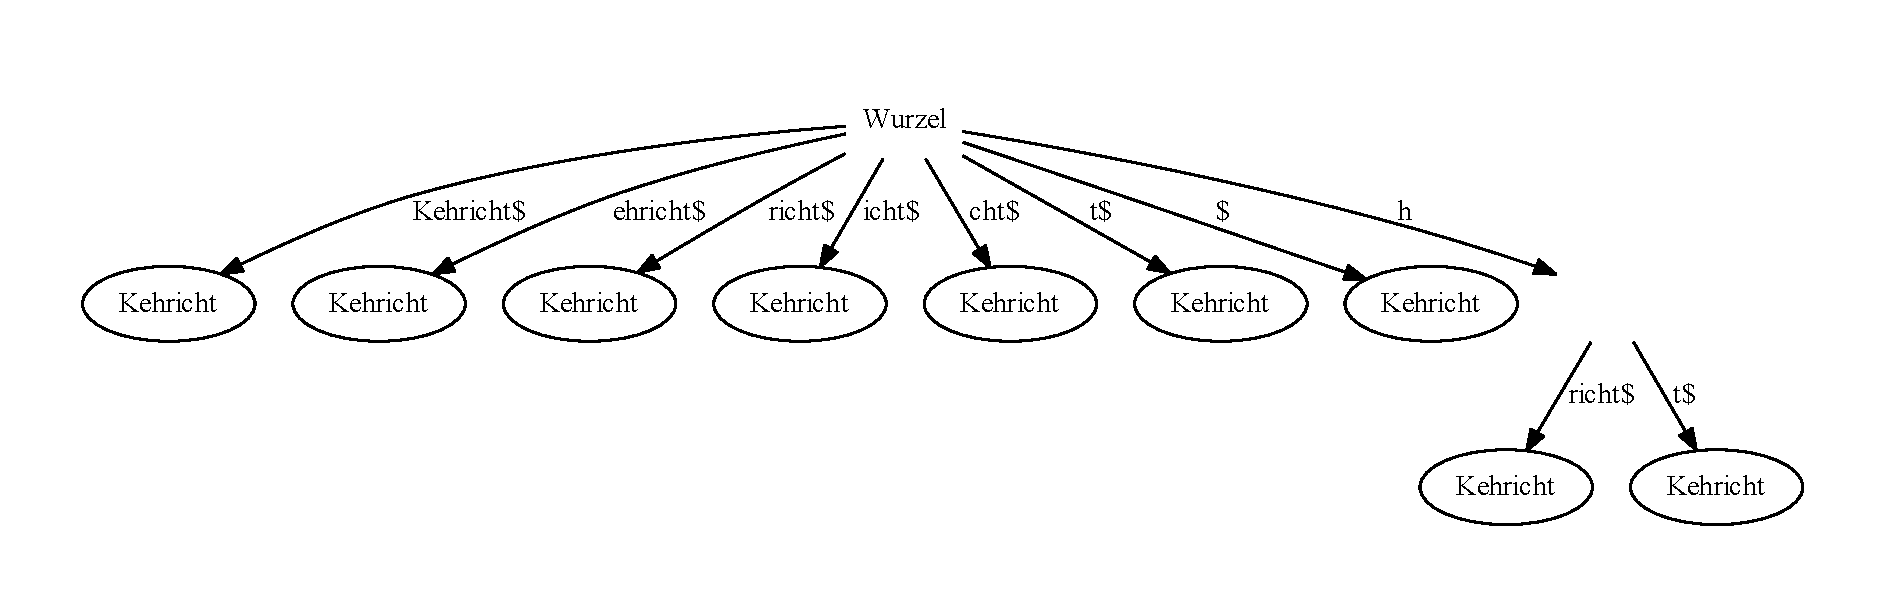
\includegraphics[scale=0.4]{resources/kehrichtSuffixTree.pdf}
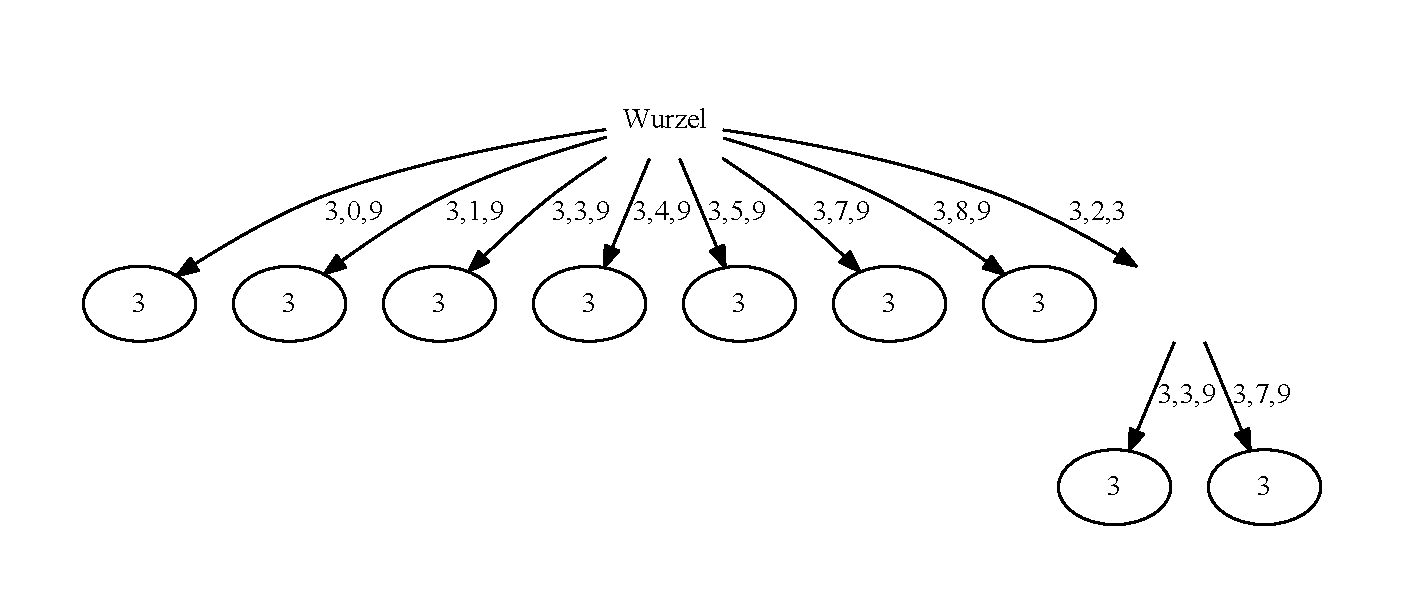
\includegraphics[scale=0.5]{resources/kehrichtCompressedSuffixTree.pdf}
\caption{\textbf{oben:} Suffixbaum  (\textit{Suffix Trie}) für das Wort "`Kehricht"'.\\\textbf{unten:} Komprimierter Suffixbaum (\textit{Suffix Tree} bzw. \textit{Compact Suffix Tree}) für das gleiche Wort. Die erste Zahl ist die ID des referenzierten Wortes, der zweite Buchstabe der Index (von 0 gezählt) des Startbuchstabens des Teilwortes, das auf dieser Kante steht und der dritte Buchstabe der Index (von 1 gezählt) des Endbuchstabens des Teilwortes, das auf der Kante steht.}
\label{fig-kehrichtSuffixTree}
\end{figure}

\paragraph{} Da Java\texttrademark keine spracheigene Implementierung eines Suffixbaumes liefert bleibt hier die Wahl des Konzepts frei. In der Literatur finden sich mehrere Vorschläge, die sich unter zwei Gesichtspunkten kategorisieren lassen:

\subsection{Aufbaualgorithmus}

\paragraph{} Die in der Literatur verbreitetsten Formen, einen Suffixbaum aufzubauen, sind die Algorithmen von Weiner, McCreight und Ukkonen in linearer Zeit (siehe auch \cite{gusfield}, S. 90). Giegerich, Kurtz und Stoye schlagen jedoch ein in der Praxis nur wenig langsameres Verfahren vor, das selbst in einer nicht-funktionellen Sprache wie Java\texttrademark lazy-evaluation\footnote{Das heißt: Die Knoten des Baumes werden erst dann evaluiert, wenn sie für eine Suchanfrage gebraucht werden und sind so lange nur implizit vorhanden.} von Suffixbäumen ermöglicht und damit deutliche Gewinne bei der Speichereffizizenz in praktischen Szenarien verspricht (siehe \cite{lazyTrees}).

\subsection{Kodierung und Kompression}

\paragraph{} Intuitiv erscheint bei der Konstruktion von Suffixbäumen eigentlich die Konstruktion eines sogenannten \textit{Suffix Trie}, also eines Suffixbaumes mit expliziten Kantenbeschriftungen (siehe auch  Definition bei Cobbs \cite{approxTreesCobbs} und Abbildung \ref{fig-kehrichtSuffixTree}, oben). Tatsächlich würde dies zu einem Speicherverbrauch von $\mathcal{O}
(n^2)$ bei einer Textlänge von $n$ führen, weshalb Techniken zur Komprimierung üblich sind. Insbesondere die Referenz auf Kantenbeschriftungen als Pointer (Edge-label-compression) ist dabei im Grunde unumstritten (siehe \cite{gusfield}, S. 104 und Abbildung \ref{fig-kehrichtSuffixTree}, unten).
Dieses Komprimierungskonzept wird auch dadurch gestützt, dass die Worte des Suchraums ohnehin für die exakte Suche in einer Hash-Tabelle indiziert werden müssen und sich daher Referenzen auf die Einträge dieser Tabelle anbieten.
\paragraph{} Weniger eindeutig allerdings ist die Lage, was weitere Komprimierungs- und Kodierungstechniken betrifft: Es erscheint auf den ersten Blick zum Beispiel naheliegend, einen Suffixbaum für den gesamten indizierten Text zu erstellen. Die genaue Reihenfolge der Worte im Text ist aber für alle Suchmodi außer der exakten Suche, die ohnehin durch Hashing gelöst werden soll, irrelevant. Demnach ist es sinnvoll, stattdessen einen generalisierten Suffixbaum zu verwenden, der nur die Worte, nicht die Vorkommen der Worte indiziert (siehe auch \cite{gusfield}, S. 116 und Abbildung \ref{fig-wolleHoldSuffixTree}).

\begin{figure}
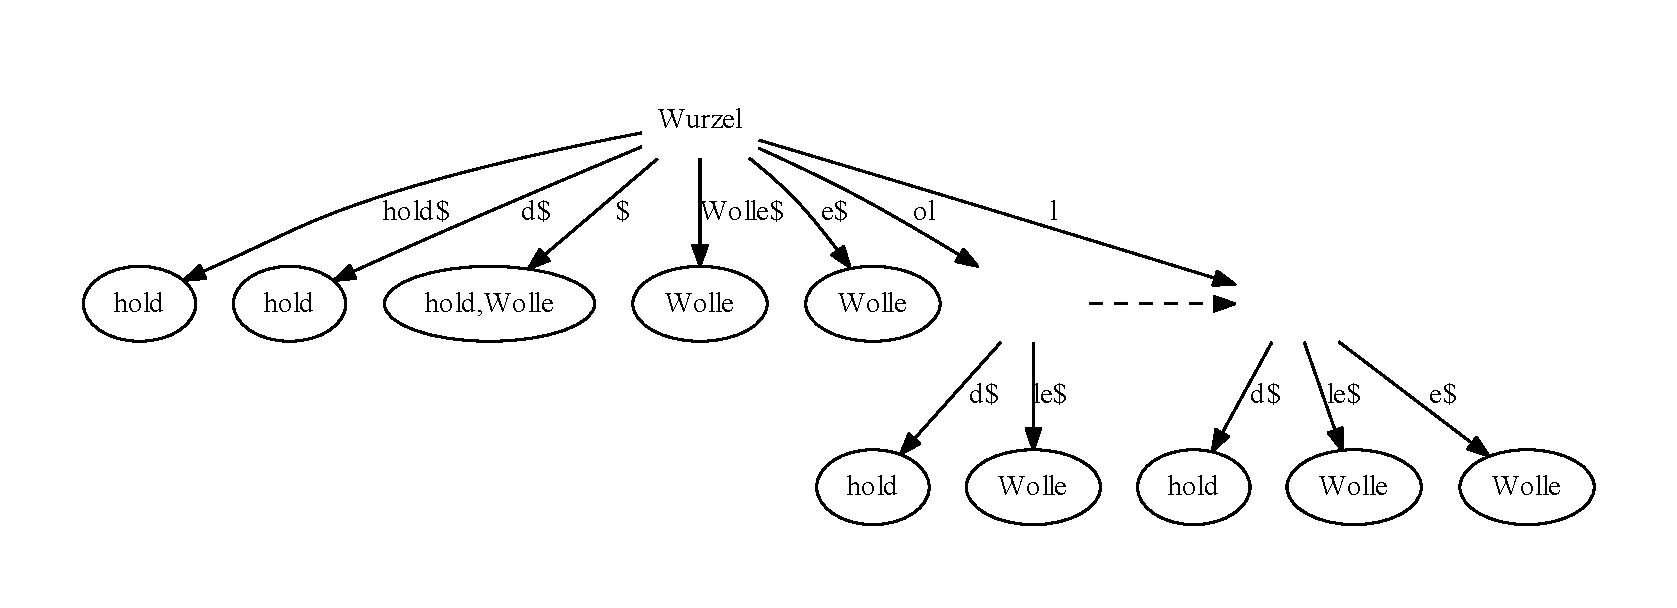
\includegraphics[scale=0.5]{resources/wolleHoldSuffixTree.pdf}
\caption{Generalisierter Suffixbaum für die Worte "`hold"' und "`Wolle"'. Für jedes Suffix beider Worte existiert je ein eindeutiger Pfad von der Wurzel zu einem Blatt, an dem alle Worte notiert sind, für die der dorthin führende Pfad ein Suffix ist. Ein Suffix-Link ist mit dem gestrichelten Pfeil angedeutet.}
\label{fig-wolleHoldSuffixTree}
\end{figure}

\paragraph{} Das allerdings erfordert Veränderungen bei zwei weiteren Konzepten: Baeza-Yates und Gonnet beschreiben das Matching von regulären Ausdrücken auf Suffixbäumen in $\mathcal{O}(n)$. Diese Technik ist nur für einen Suffixbaum über den gesamten Text beschrieben. Hier müsste außerdem der Inhalt des Suffixbaumes binär kodiert werden (siehe \cite{baeza-yates}).
\paragraph{} Ebenso verhält es sich bei der inexakten Suche: Die modernste Variante zur Lösung des Problems in Suffixbäumen (siehe Überblick in \cite{approximateIndexing}) wird von Cobbs als Weiterentwicklung eines Algorithmus von Ukkonen und Jukinen vorgestellt (siehe \cite{approxTreesUkkonen1,approxTreesUkkonen2,approxTreesCobbs}). Sie ist aber ebenfalls nur für einen Suffixbaum über den gesamten Text beschrieben.

\subsection{Auswahl des Konzepts}

\paragraph{} Die Nutzung eines Suffixbaums mit lazy evaluation erscheint zwar reizvoll, würde aber Laufzeitverluste für die Suchanfragen von Nutzenden bedeuten, weil zusätzlich zur Laufzeit der Suche die Knoten des Baums evaluiert werden müssten. Daher wird im weiteren Verlauf stattdessen der Algorithmus von Ukkonen zum Aufbau des Baumes verwendet (siehe \cite{gusfield}, S. 94-107 bzw. im Original \cite{ukkonen}).
\paragraph{} Dennoch soll durch Nutzung eines generalisierten Suffixbaums eine möglichst speichereffiziente Lösung erstellt werden. Das bedeutet jedoch, dass die vorgestellten Suchkonzepte für reguläre Ausdrücke und inexaktes Matching adaptiert werden müssen und vielleicht nur mit Einschränkungen nutzbar sind.

\section{Endliche Automaten}
\label{meth-automata}

\paragraph{} Ein endlicher Automat besteht aus einer Menge von Zuständen, zwischen denen sich der Automat je nach Eingabe bewegt. Das besondere Kennzeichen endlicher Automaten ist, dass die Folgezustände nur mittels des momentanen Zustandes und des Inputs berechnet werden können (siehe auch \cite{automata}, S. 37f.).
\paragraph{} Bei der Bearbeitung von regulären Ausdrücken schlagen Baeza-Yates und Gonnet die Nutzung von deterministischen, endlichen Automaten (DEA) vor \cite{baeza-yates}. Solche Automaten haben im Aufbau unter Umständen exponentiellen Zeit- und Platzverbrauch abhängig vom Suchmuster (siehe \cite{automata}, S. 60). Daher erscheint es wünschenswert, stattdessen auf nichtdeterministische endliche Automaten (NEA) zurückzugreifen, solange das die eigentliche Suchzeit nicht zu weit erhöht.

\section{Scoring}
\label{meth-scoring}

\paragraph{} Zwar gibt es in der Literatur einige Ausführungen zur Sortierung von Suchergebnissen, diese befassen sich allerdings in der Regel nicht mit den Inhalten einer einzelnen Homepage sondern betrachten die Domäne der großen Internetsuchmaschinen. Solche Techniken sind im Allgemeinen für den hiesigen Fall ungeeignet, weil sie auf Links \textit{zwischen} Seiten aufbauen (siehe \cite{google}), während \textit{BiBiServSearch} nur \textit{innerhalb} einer Seite sucht.
\paragraph{} Für die vorliegende Domäne ist deshalb ein simpleres Konzept angebracht. Zwei Maßstäbe für das Scoring liegen nahe:
\begin{enumerate}
 \item Ergebnisse einer Suche sind Dokumente. Ein Dokument kann viele verschiedene Vorkommen von Matches für das Suchmuster enthalten. Es kann davon ausgegangen werden, das Dokumente, die mehr Vorkommen enthalten, auch eher diejenigen Dokumente sind, die für Nutzende interessant erscheinen (\textbf{Primärscore}).
 \item Bei Teilwort- und inexakter Suche können sich Matches unter Umständen stark vom Suchmuster unterscheiden (im Extremfall z.B. könnten Nutzende nach dem englischen, unbestimmten Artikel "`a"' suchen und bekämen bei der Teilwortsuche auch das Match "`Donaudampfschiffkapitän"' angezeigt). Hier bieten sich wiederum zwei Kriterien für die Bewertung an (\textbf{Sekundärscore}):
\begin{enumerate}
 \item Wie viel länger ist das Match als die tatsächlich mit dem Suchmuster übereinstimmende Sequenz des Wortes?
 \item Mussten Methoden der inexakten Suche angewandt werden?
\end{enumerate}
\end{enumerate}

\paragraph{} Der Sekundärscore ist im Allgemeinen ein ungenaueres Kriterium als das erste Maß (z.B. erscheinen bei einer Suche nach dem Wort "`hold"' die Matches "`holder"' und "`holde"' ja gleich relevant, obwohl Match und die mit dem Suchmuster übereinstimmende Sequenz nicht gleich lang sind). Daher wird hier eine starke Priorisierung des Primärscores verwendet: Dokumente werden zuerst nach dem Primärscore sortiert und erst bei gleichem Primärscore wird nach dem Sekundärscore sortiert.

\newpage

\section{Vergrößern und Verkleinern des Suchraums}
\label{meth-addAndRemove}

\paragraph{} Das Vergrößern und Verkleinern des Suchraums (d.h.: Das Einfügen und Entfernen von Tools auf dem \textit{BiBiServ2} durch Administratoren) betrifft nach dem bisherigen Konzept zwei Datenstrukturen: Die Hashing-Tabellen und den Suffixbaum.
\paragraph{} Die Hashing-Tabellen erscheinen dabei unproblematisch: Einfügen und Entfernen von Worten, Vorkommen und Dokumenten ist jeweils in konstanter Zeit möglich (siehe \ref{meth-hashing}). Auch die Synchronisation ist hier trivial lösbar: Einzelne Such-, Einfügungs- und Entfernungsanfragen können durch gegenseitigen Ausschluss synchronisiert werden.
\paragraph{} Weniger einfach ist der Fall beim Suffixbaum: Zwar bieten Cham, Hon, Lam und Sadakane ein Suffixbaum-Konzept an, aus dem sich dynamisch Einträge entfernen lassen (siehe \cite{dynamicTrees}), allerdings steigt die Zeit für Suchanfragen auf $\mathcal{O}(m \cdot log(n))$ bei einer Musterlänge $m$ und Textlänge $n$. Diese Abhängigkeit von der Textlänge ist angesichts der geforderten geringen Antwortzeiten für Suchanfragen unvertretbar.
\paragraph{} Dementsprechend muss ein Entfernen von Elementen aus dem Suffixbaum umgangen werden. Hilfreich ist hier, dass nach einem Suchvorgang ohnehin noch auf die Hash-Tabellen zugegriffen werden muss (um alle Vorkommen der Matches zu finden) und dementsprechend Suchergebnisse aus dem Suffixbaum, die in den Hash-Tabellen nicht mehr gespeichert sind, einfach ignoriert werden können. Um trotzdem zu verhindern, dass alte Einträge den Arbeitsspeicher blockieren, sollte der Suffixbaum in regelmäßigen Abständen neu aufgebaut werden.
\paragraph{} Ein weiteres Problem stellt sich beim Einfügen neuer Einträge: Das ist mit Ukkonens Algorithmus zwar mit leichten Variationen möglich (siehe \cite{gusfield}, S. 116), würde jedoch den Suffixbaum währenddessen blockieren. Daher liegt es hier nahe, eine Kopie des Baums anzulegen, in die Kopie des Baums neue Worte einzufügen und dann den alten Baum durch die Kopie zu ersetzen\footnote{Dieser Ersetzungsprozess bedeutet nur die Umschaltung einer Referenz. Hier erfolgt ein schreibender Zugriff, währenddessen Suchanfragen blockiert werden müssen. Dieser Zugriff ist allerdings in konstanter Zeit möglich und deshalb vertretbar. Dieses Konzept stammt in weiten Teilen von Jan Krüger (persönliches Gespräch, August 2012).}. Eine weitere Modifikation löst auch das Problem einer vormaligen Verkleinerung des Suchraums: Beim Einfügen neuer Dokumente wird nicht eine Kopie des aktuellen Baumes angelegt, sondern der Baum wird aus der aktuellen Wort-Hash-Tabelle neu aufgebaut. Die Bearbeitung vormaliger Entfernungsanfragen wird somit bei einer Neueinfügung von Dokumenten nachgeholt.


\chapter{Implementierung}
\label{implementierung}

\paragraph{} In diesem Kapitel ist die Umsetzung der in Kapitel \ref{methoden} vorgestellten Konzepte und Methoden beschrieben. Das schließt sowohl die Architektur der Implementierung (siehe \ref{impl-architecture}) als auch eine detaillierte Beschreibung der Algorithmen ein, wie sie im fertigen Programm vorliegen (siehe \ref{impl-algorithms}).

\section{Systemarchitektur}
\label{impl-architecture}

\paragraph{} Die fertige Systemarchitektur entspricht weitgehend dem vorgeschlagenen Konzept (siehe Anhang \ref{uml-architecture}). Das System gliedert sich vornehmlich in folgende Bereiche:
\begin{enumerate}
\item Das Hauptpaket liefert die API für alle Anfragen an das Programm und leistet den Import von Dokumenten (siehe \ref{arch-import}).
\item Hilfsklassen für das Hauptpaket übernehmen die Einteilung von Suchanfragen in Suchmodi, erledigen exakte Suchanfragen und kümmern sich um die Sortierung aller Suchergebnisse (siehe \ref{arch-helper}).
\item Das Indexpaket bildet Dokumente, Worte und Vorkommen in einer Indexstruktur ab (siehe \ref{arch-index}).
\item Die Worte werden ebenfalls in einem Suffixbaum gespeichert, um damit Suchanfragen in den übrigen Modi zu bearbeiten (siehe \ref{arch-suffix}).
\item Ein Tochterpaket des Suffixbaum-Pakets enthält die Feinumsetzung von Suchanfragen in Semantik und die Unterstützung des eigentlichen Matchings (siehe \ref{arch-pattern}).
\end{enumerate}

\paragraph{} Zusätzlich existieren noch die Pakete \texttt{results}, \texttt{exceptions}, \texttt{util} und \texttt{xmltools} zu Unterstützungszwecken. Im Anhang ist die Paketstruktur auch in einem UML-Paketdiagramm visualisiert (siehe \ref{uml-package}).

\paragraph{} Im Folgenden werden die wichtigsten Pakete und Klassen des Systems beschrieben. Genauere Informationen über die einzelnen Methoden und Attribute sind im JavaDoc\texttrademark des Programms enthalten. Eine grafische Übersicht liefert das Klassendiagramm im Anhang (siehe \ref{uml-classes}).

\subsection{Import und Schnittstelle}
\label{arch-import}

\paragraph{} Für Anfragen von außen steht das Hauptpaket, \texttt{de.unibi.cebitec.bibiserv.\\search} zur Verfügung. Alle Anfragen - Einfügen und Entfernen von Dokumenten in den Suchraum sowie die Suche selbst - können hierüber angestoßen werden. Auch alle Rückgabewerte der entsprechenden Methoden werden in Instanzen dieses Pakets ausgedrückt. Für den Import wird dabei auf das "`Apache Tika"'-Paket\footnote{siehe \url{http://tika.apache.org/}} zurückgegriffen. Damit ist es möglich, alle für den \textit{BiBiServ2} relevanten Dokument-Typen zu bearbeiten (siehe auch \ref{intro-compatibility}).

\subsubsection{Search}
\label{arch-search}

\paragraph{} Mit ihrer Tochterklasse \texttt{BiBiServSearch} bildet \texttt{Search} beinahe die gesamte API der Anwendung. Hierüber werden alle wesentlichen Befehle von außen angestoßen. Die wichtigsten Methoden sind:

\paragraph{getInstance:} Gibt die einzige Instanz der search-Klasse zurück.

\paragraph{addDocuments:} Fügt neue Dokumente in den Suchraum ein (siehe auch \ref{algo-addDoc}).

\paragraph{search:} Stößt eine Suche für das gegebene Suchmuster an und gibt anschließend eine sortierte Liste mit Suchergebnissen zurück. Details dazu sind im Kapitel \ref{impl-algorithms} zu finden.

\paragraph{removeDocument:} Entfernt ein Dokument anhand seiner URL (siehe auch \ref{algo-removeDoc}).

\subsubsection{OutputSearchResult}

\paragraph{} Diese Klasse repräsentiert ein Suchergebnis. Es enthält die URL des Dokuments, in dem das Suchmuster gefunden wurde und eine (unsortierte) Liste von Treffern, die für das Suchmuster im Dokument gefunden wurden. Diese Treffer können Nutzenden dann angezeigt werden (siehe auch Abbildung \ref{fig-matches-screenshot}).

\newpage

\subsection{Hilfsklassen für Suchvorgänge}
\label{arch-helper}

\paragraph{} Im Hintergrund des Hauptpaketes wirken für Vor- und Nachbereitung von Suchanfragen sowie die Bearbeitung der exakten Suche einfache Hilfsklassen. Die wichtigsten davon sind hier vorgestellt.

\subsubsection{SearchQuery}

\paragraph{} Diese Klasse repräsentiert eine Suchanfrage. Sie enthält den Typ der Suchanfrage (Exakte Suche, Teilwortsuche oder Inexakte Suche, siehe auch \ref{anforderungen-features}) sowie die Worte, nach denen gesucht werden soll. Ihre wichtigste Methode ist:

\paragraph{parseQuery:} Mit dieser statischen Methode wird aus einem Eingabestring eine Instanz der \texttt{SearchQuery}-Klasse erzeugt.

\subsubsection{SearchScore}

\paragraph{} Ein \texttt{SearchScore}-Objekt repräsentiert die Wertung eines Suchergebnisses. Die wichtigste Methode hier ist:

\paragraph{calculateScoredResults:} Diese statische Methode sortiert eine Liste von Suchergebnissen nach "`Relevanz"'. Die Details zur Bewertung von Suchergebnissen sind in Kapitel \ref{algo-scoring} beschrieben.

\subsubsection{ExactMatcher}

\paragraph{} Eine \texttt{ExactMatcher}-Instanz kann für ein gegebenes Array von Worten eine exakte Suche durchführen, bei der die Worte in genau dieser Reihenfolge gesucht werden.

\paragraph{getMatches:} Startet den eigentlichen Suchvorgang und gibt etwaige Treffer zurück.

\subsection{Indexstruktur}
\label{arch-index}

\paragraph{} Das in Kapitel \ref{meth-hashing} beschriebene Hashing findet im Paket \texttt{de.unibi.cebitec.\\bibiserv.search.index} statt. Üblicherweise werden dabei Datensätze über eine eindeutige ID referenziert. Dies dient zur Reduzierung des Speicherverbrauchs, weil die IDs eine feste Größe besitzen. Im Einzelnen sind die Schlüssel-Wert-Kombinationen wie folgt:

\paragraph{}

\begin{tabularx}{\textwidth}{llX}
\hline
\textbf{Klasse} & \textbf{Argument-Klasse} & \textbf{Wert-Klasse} \\ [0.1cm]
\hline
MainIndex & WordID & OccurenceSet \\ [0.1cm]
\hline
BiBiServDocument & DocumentID & BiBiServDocument \\ [0.1cm]
\hline
WordIndex & String & WordID \\ [0.1cm]
\hline
\end{tabularx}

\paragraph{} Alle Indizes sind Instanzen der Klasse \texttt{de.unibi.cebitec.bibiserv.search.\\util.Index}. Diese Klasse erweitert allerdings lediglich die übliche \texttt{HashMap} um Synchronisierungsmethoden, um thread-sicheren Zugriff zu ermöglichen. Die Index-Klassen, die hier vorgestellt werden, stellen jeweils nur statische Methoden zur Verfügung, da jeder Index nur einmal im Speicher liegen soll.

\subsubsection{Occurence}

\paragraph{} Diese Klasse implementiert das Vorkommen eines Wortes. Ein Vorkommen referenziert die ID des Wortes, dessen Vorkommen es ist, die ID des Dokuments, in dem es vorkommt, sowie den eigenen Vorgänger und Nachfolger im indizierten Text (Im Text "`der holde Knabe"' wäre der Vorgänger des Vorkommens des Wortes "`holde"' z.B. ein bestimmtes Vorkommen des Wortes "`der"'). Dabei wird die Referenzierung von Vorgängern und Nachfolgern bei Vorkommen sowohl für die exakte Suche benutzt (siehe \ref{algo-exact}) als auch für die Darstellung von Suchergebnissen für Nutzende des Programms: Auf der Ergebnisseite wird nicht nur das Suchergebnis selbst, sondern auch die Umgebung des Treffers angezeigt (siehe Abbildung \ref{fig-matches-screenshot}).

\subsubsection{MainIndex}
\label{arch-mainIndex}

\paragraph{} Der Hauptindex beantwortet die Suchanfragen der Search-Klasse und bildet die IDs von Worten auf eine Menge von Vorkommen dieser Worte ab. Die wesentlichen Funktionen dieser Klasse sind:

\paragraph{indexOccurence:} Indiziert das Vorkommen eines Wortes bei der Neueinfügung eines Dokuments.

\paragraph{searchExactly:} Sucht die Vorkommen eines Wortes in seiner exakten Schreibweise aus dem Index heraus. Die genaue Funktionsweise wird näher in Kapitel \ref{algo-exact} beschrieben.

\paragraph{searchSuperStrings:} Reicht eine Suchanfrage an den Suffixbaum weiter.

\paragraph{getOccurencesForWordID:} Gibt alle Vorkommen eines Wortes mit der gegebenen ID zurück. Dies ist die eigentliche Indexfunktion des Hauptindex und wird bei allen Suchanfragen benutzt.

\paragraph{removeDocumentReferencesByID:} Es werden alle Wortvorkommen aus dem Index entfernt, die zum Dokument mit der gegebenen ID gehören.

\subsubsection{WordIndex}
\label{arch-wordIndex}

\paragraph{} Der Wortindex ist dazu da, sowohl in einem Verzeichnis von Worten als auch im Suffixbaum alle Worte einzufügen, die indiziert werden. Der Index selbst bildet Worte auf ihre jeweilige ID ab. Der umgekehrte Weg (also die Abbildung von Wort-IDs auf Worte) ist ebenfalls an vielen Stellen nötig, wird aber über einen Pointer in den WordIDs selbst erledigt. Die wichtigsten Funktionen dieser Klasse sind:

\paragraph{indexWord:} Fügt ein Wort in den Index ein (sofern es noch nicht indiziert ist) und gibt die (ggf. neu erzeugte) ID des Wortes zurück.

\paragraph{getTreeInstance:} Diese Funktion stellt den Suffixbaum nach außen hin zur Verfügung. Die Bauminstanz wird zum Beispiel vom Hauptindex zur Beantwortung von Suchanfragen benötigt.

\paragraph{getID:} Gibt die ID eines gegeben Wortes zurück oder \texttt{null}, falls das Wort nicht indiziert ist.

\paragraph{removeWord:} Entfernt (mit den beiden Schwesterfunktionen \texttt{removeWordByID} und \texttt{removeWordByReference}) Worte aus dem Index. Das kommt dann vor, wenn Dokumente aus dem Index entfernt werden.

\subsubsection{SuffixTreeAppendSession}
\label{arch-session}

\paragraph{} Diese Klasse ermöglicht das Einfügen von Worten in den Suffixbaum. Das setzt das in Abschnitt \ref{meth-addAndRemove} vorgeschlagene Synchronisationssystem um. Die API-Methoden für eine solche Session sind:

\paragraph{open:} Öffnet eine Session, in der Worte zum Suffixbaum hinzugefügt werden können. Dabei wird aus dem momentanen Wort-Index der aktuelle Suffixbaum als Kopie neu aufgebaut. Es wird auch sichergestellt, dass nur eine Session gleichzeitig offen ist.

\paragraph{appendWordToTree:} Fügt das Wort mit der gegebenen ID in den Suffixbaum ein.

\paragraph{close:} Schließt die momentane Session. Das heißt, dass der alte Suffixbaum durch die Kopie dieser Session ersetzt wird.

\subsubsection{BiBiServDocument}
\label{arch-docIndex}

\paragraph{} Diese Klasse dient als Repräsentation von Dokumenten für die Suche. Ein Dokument referenziert ein URL-Suffix, über das sein Inhalt auf der Homepage des \textit{Bielefeld Bioinformatics Service} erreichbar ist, und seine Dokumenten-ID. Gleichzeitig enthält die Klasse den Dokumenten-Index, der Dokumenten-IDs auf eigentliche \texttt{BiBiServDocument}-Instanzen abbildet. Die wichtigsten Funktionen sind:

\paragraph{createIndexedDocument:} Erzeugt eine neue \texttt{BiBiServDocument}-Instanz für einen gegebenen Dateinamen und fügt sie in den Index ein.

\paragraph{getDocumentByID:} Gibt die \texttt{BiBiServDocument}-Instanz für die gegebene ID zurück.

\paragraph{removeDocumentByIdentifier:} Entfernt das erste Dokument aus dem Index, das das gegebene URL-Suffix hat und gibt den Löschauftrag auch an den Hauptindex weiter. Es wird hier nur das erste Dokument gelöscht, weil die Suffixe eindeutig sein müssen - sonst könnten die Websites auf dem \textit{BiBiServ2} nicht eindeutig referenziert werden.

\subsection{Suffixbaum}
\label{arch-suffix}

\paragraph{} Das Paket \texttt{de.unibi.cebitec.bibiserv.search.suffixtree} enthält alle \\Klassen, die zum Aufbau des Suffixbaumes nötig sind. Näheres zur algorithmischen Seite des Aufbaus des Suffixbaums ist in Kapitel \ref{algo-suffix} zu lesen.
\paragraph{} Einige Klassen entsprechen dabei ganz direkt Konzepten des Suffixbaums:
\begin{itemize}
\item \textbf{SuffixTreeEdge:} Implementiert eine Kante des Suffixbaums.
\item \textbf{SuffixTreeLeaf:} Implementiert ein Blatt des Suffixbaums.
\item \textbf{SuffixTreeSplitNode:} Implementiert einen internen Knoten des Suffixbaums.
\end{itemize}

\subsubsection{SuffixTree}

\paragraph{} Dies ist die Klasse, die hauptsächlich bei äußeren Zugriffen auf das Paket benutzt werden sollte. Sie stellt Zugriffsfunktionen für alle Szenarien zur Verfügung, die für diese Anwendung eine Rolle spielen. Die wichtigsten Funktionen sind:

\paragraph{appendToTree:} Fügt das Wort mit der gegebenen ID in den Suffixbaum ein. Auf diese Methode wird nicht direkt, sondern nur über eine Session (siehe Abschnitt \ref{arch-session}) zugegriffen.

\paragraph{getAllMatches:} Sucht die IDs aller Worte heraus, die ein Teilwort besitzen, das dem Suchmuster entspricht. Die Sprache für solche Suchmuster ist auch in Kapitel \ref{algo-pattern-language} beschrieben. Das Suchmuster wird seinerseits zu einem NEA umgewandelt (siehe auch \ref{meth-automata}, \ref{arch-pattern} und \ref{algo-regex}). Für den Suchvorgang selbst wird implizit ein SuffixTreeMatcher (siehe auch \ref{suffixTreeMatcher}) erzeugt.

\subsubsection{SuffixTreeCharacter}

\paragraph{} Für den Aufbau von Suffixbäumen ist es nötig, ein unverwechselbares Endzeichen zu haben (in der Literatur meist als \texttt{\$} notiert (siehe auch \cite{gusfield}, S. 91). Diese Hüllklasse für den primitiven Datentyp \texttt{char} wurde implementiert, um sicherzustellen, dass solch ein Zeichen existiert.

\subsubsection{SuffixTreeConstructor}

\paragraph{} Diese Klasse übernimmt den eigentlichen Aufbau des Suffixbaums gemäß Ukkonens Algorithmus. Mehr dazu ist in Kapitel \ref{algo-suffix} zu lesen. Für äußere Zugriffe ist nur die Methode \textbf{constructTree} relevant, die den Konstruktionsprozess anstößt.

\subsection{Suffixbaum-Suchmuster}
\label{arch-pattern}

\paragraph{} Das Paket \texttt{de.unibi.cebitec.bibiserv.search.suffixtree.pattern} enthält alle Klassen, die sich direkt auf die Algorithmen zum Auffinden von Suchmustern im Suffixbaum beziehen. Die Details dieser Algorithmen sind im Kapitel \ref{impl-algorithms} beschrieben. Hier sind nur in aller Kürze die wichtigsten Klassen dokumentiert.

\subsubsection{PatternChar}

\paragraph{} Die Töchter dieser abstrakten Klasse repräsentieren einzelne, "`semantische Zeichen"' eines Suchmusters, insbesondere bei der Verwendung von regulären Ausdrücken. "`Semantisches Zeichen"' bedeutet: Ein solches Zeichen prüft in einem Suchvorgang \textit{genau ein} tatsächliches Referenzzeichen. Ein Referenzzeichen wird genau dann akzeptiert, wenn es in der regulären Sprache liegt, die vom \texttt{PatternChar} definiert wird. Beispielsweise definiert \texttt{[abc]} als \texttt{OneOfPattern-\\Char} die Sprache $\lbrace a, b,c\rbrace$. Die wichtigsten Methoden dieser Klassen sind:

\paragraph{matchSingleCharacter:} Prüft, ob ein einzelnes Zeichen in der regulären Sprache dieses \texttt{PatternChars} liegt oder nicht.

\paragraph{getMatchingCharacters:} Teilt eine Menge von Referenzzeichen auf in die Menge derjenigen Zeichen, die in der regulären Sprache dieses \texttt{PatternChar} liegen, und alle übrigen Zeichen. Beide Mengen werden in einem Tupel zurückgegeben.

\paragraph{findSuperSet:} Prüft für sich selbst und einen anderen \texttt{PatternChar}, ob die eigene reguläre Sprache eine Obermenge der Sprache des anderen \texttt{PatternChar} ist (und/oder umgekehrt) und gibt, falls dem so ist, den entsprechenden \texttt{Pattern-\\Char} zurück. Zum Beispiel würde bei der Eingabe der \texttt{PatternChars} \texttt{[ab]} und \texttt{[abc]} \texttt{[abc]} zurückgegeben, weil die Sprache von \texttt{[abc]} alle Zeichen der Sprache von \texttt{[ab]} enthält und noch mehr. Falls keine der beiden Sprachen eine Obermenge der jeweils anderen ist wird \texttt{null} zurückgegeben.

\subsubsection{RegexParser}

\paragraph{} Diese abstrakte Klasse stellt allgemeine Methoden zur Verfügung, um Strings, die reguläre Ausdrücke repräsentieren, zu verarbeiten. Der Parse-Vorgang entspricht dabei einem Transduktor, also einem endlichen Automaten, der einen String einliest und etwas anderes ausgibt (in diesem Fall einen NEA für den regulären Ausdruck dieses String; siehe auch \cite{jurafsky&martin}, S. 71).
\paragraph{} Der Parser gibt die gefundenen \texttt{PatternChars} an die instanziierende Klasse weiter, wo sie verarbeitet werden können. Dabei wird nur zwischen \texttt{Pattern-\\Chars}, die einem \texttt{*} vorangehen (also beliebig oft vorkommen dürfen) unterschieden und solchen, die es nicht tun. Details dieser Sprache werden in Kapitel \ref{algo-pattern-language} beschrieben.

\subsubsection{SearchPattern}

\paragraph{} Instanzen dieser Klasse entsprechen einem Suchmuster, das von Nutzenden eingegeben wurde. Die Implementierung entspricht einem NEA (siehe auch Abbildung \ref{fig-nea}). Wie diese Automaten für die Suchvorgänge verwendet werden ist in Kapitel \ref{algo-regex} beschrieben.


\subsubsection{SuffixTreeMatcher}
\label{suffixTreeMatcher}

\paragraph{} Der \texttt{SuffixTreeMatcher} erledigt die Suchaufträge eines Suffixbaumes. Dabei arbeitet er mit Instanzen der internen Klasse \texttt{MatchingState}, die den momentanen Status des Suchvorganges repräsentieren. Die Details dieses Algorithmus sind in Kapitel \ref{algo-regex} beschrieben.

\paragraph{getAllMatches} ist dabei die zentrale Methode des \texttt{SuffixTreeMatchers}, mit der für den gegebenen Knoten des Baums und das gegebene Suchmuster alle Worte herausgesucht werden können, die dem Suchmuster entsprechen.

\newpage

\section{Algorithmen und Abläufe}
\label{impl-algorithms}

\paragraph{} In diesem Kapitel soll es darum gehen, die genauen Abläufe innerhalb des Programms zu beschreiben. Damit sind vier verschiedene Vorgänge gemeint:
\begin{enumerate}
 \item Das Einfügen neuer Dokumente in den Suchraum (siehe \ref{algo-addDoc})
 \item Die eigentlichen Suchalgorithmen
 \item Die Bewertung der Suchergebnisse (siehe \ref{algo-scoring})
 \item Das Entfernen von Dokumenten aus dem Suchraum (siehe \ref{algo-removeDoc})
\end{enumerate}

\paragraph{} Bei Suchanfragen wird analog zur Anforderungsanalyse in Abschnitt \ref{anforderungen-features} zwischen drei verschiedenen Suchmodi unterschieden: Der exakten Suche (siehe \ref{algo-exact}), der Teilwortsuche (siehe \ref{algo-substring}), und der inexakten Suche (siehe \ref{algo-inexact}). Bei den beiden letztgenannten Varianten ist zudem eine Suche mit Hilfe von regulären Ausdrücken möglich (siehe \ref{algo-regex}).
\paragraph{} Mit welcher Syntax Nutzende Suchanfragen eingeben können ist in Abschnitt \ref{algo-pattern-language} beschrieben.

\subsection{Einfügen eines Dokuments}
\label{algo-addDoc}

\paragraph{} Beim Einfügen eines Dokuments in den Suchraum wird in den folgenden Schritten vorgegangen:
\begin{enumerate}
 \item Indiziere das Dokument und seinen Inhalt in den Hash-Tabellen.
 \item Füge den Inhalt in den Suffixbaum ein.
\end{enumerate}

\subsubsection{Indizierung}
\label{algo-index}

\paragraph{} Bei der Indizierung eines Dokuments wird zuerst das Dokument selbst im Dokumenten-Index abgelegt. Dann bearbeitet das Programm den Inhalt des Dokuments. Dabei wird zeilenweise der Dokumenteninhalt gelesen und die Zeilen dann ihrerseits in Worte unterteilt. Dabei orientiert sich die Definition eines "`Wortes"' hier an der Programmiersprache Java: Ein Wort ist jede Zeichenkette, die aus Elementen der Menge $\lbrace$a,b,$\dots$,z,A,B,$\dots$,Z,0,1,$\dots$,9,ä,ö,ü,Ä,Ö,Ü,ß$\rbrace$ besteht\footnote{ Dabei werden in der Vorverarbeitung alle Kleinbuchstaben in Großbuchstaben umgesetzt. Es ist hier also ein Alphabet fixer Größe mit $26 + 10 + 4 = 40$ Zeichen implementiert.}. Alle übrigen Zeichen werden ignoriert\footnote{ Es wird hier heuristisch vermutet, dass jedes andere Zeichen ein Wortbegrenzer ist. Für die Suche führt die Heuristik zu keinen Nachteilen, weil bei der Vorverarbeitung der Suchanfrage ebenfalls alle Zeichen, die nicht im definierten Alphabet liegen, gelöscht werden und Nutzende deshalb trotzdem die gewünschten Suchergebnisse bekommen. Im schlimmsten Falle ist lediglich das Scoring der Ergebnisse verwirrend.}. Das im Englischen gebräuchliche "`don't"' beispielsweise wird hier eigentlich als zwei Worte interpretiert: "`don"' und "`t"'. Außerdem werden die Worte immer als großgeschrieben interpretiert und indiziert.
\paragraph{} Jedes Wort wird im Wortindex eingefügt (wenn es nicht bereits im Index liegt) und schließlich wird jedes Vorkommen des Wortes im Hauptindex indiziert. In Pseudocode gegossen entspricht das Algorithmus \ref{code-insert}.

\begin{algorithm}
\caption{Indizieren eines neuen Dokuments}
\label{code-insert}
\begin{algorithmic}
\STATE{Erzeuge eine neue Dokumenten-ID $i_d$ für das Dokument $d$ und füge einen Eintrag im Dokumenten-Index ein.}
\FORALL{Worte $w$ in $d$}
	\IF{$w$ is im Wortindex enthalten}
		\STATE{Hole die entsprechende Wort-ID $i_w$ aus dem Index.}
	\ELSE
		\STATE{Erzeuge eine neue Wort-ID $i_w$ und füge einen Eintrag im Wortindex ein.}
	\ENDIF
	\STATE{Füge $w$ in den Suffixbaum ein.}
	\IF{$i_w$ ist im Hauptindex enthalten}
		\STATE{Hole die entsprechende Menge von Vorkommen $V$ aus dem Index.}
	\ELSE
		\STATE{Erzeuge eine neue, leere Menge von Vorkommen $V$ und füge einen Eintrag im Hauptindex ein.}
	\ENDIF
	\STATE{Füge ein neues Vorkommen $v$ für die Dokumenten-ID $i_d$ und die Wort-ID $i_w$ in $V$ hinzu.}
	\IF{$v'$ ist gesetzt}
		\STATE{Setze den Nachfolger von $v'$ auf $v$ und den Vorgänger von $v$ auf $v'$.}
	\ENDIF
	\STATE{Setze $v'$ $=$ $v$.}
\ENDFOR
\end{algorithmic}
\end{algorithm}

\subsubsection{Aufbauen des Suffixbaums}
\label{algo-suffix}

\paragraph{} Das Einfügen eines Wortes in den Suffixbaum geschieht im wesentlichen gemäß Ukkonens Algorithmus wie bei Gusfield beschrieben (siehe \cite{gusfield}, S. 94-107 bzw. im Original \cite{ukkonen}). Aus Platzgründen kann hier die Beschreibung nicht im Detail wiederholt werden. Allerdings ist eine Skizze der vorliegenden Implementierung des Algorithmus im Anhang \ref{ukkonen} angefügt. Hier seien lediglich einige Feinheiten genannt:
\paragraph{} Vor allem nutzt \textit{BiBiServSearch} - wie schon in Kapitel \ref{arch-suffix} angemerkt - keinen einfachen, sondern einen generalisierten Suffixbaum. Dabei wird insbesondere an den Blättern nicht nur, wie bei Gusfield (siehe \cite{gusfield}, S. 116-119), \textit{ein} Wort notiert, für das der hinführende Pfad ein Suffix ist, sondern \textit{alle} Worte, für die das gilt (siehe auch Abbildung \ref{fig-wolleHoldSuffixTree}).
\paragraph{} Ferner muss es möglich sein, auch nachträglich Worte in den Baum einzufügen. Das führt zu zwei  Sonderfällen:
\begin{itemize}
 \item \textbf{Ein neues Wort $w$ ist ein echtes Präfix eines bereits eingefügten Wortes $w'$:} In diesem Fall können Probleme dadurch behoben werden, dass genau dann ein mismatch beim Einfügen in den Baum auftritt, wenn $w$ endet. Dann folgt das Endzeichen $\$$, das in $w'$ an dieser Stelle nicht auftrat. Hier können nun die nötigen split-Operationen vorgenommen werden.
 \item \textbf{Ein neues Wort $w$ ist ein Suffix eines bereits eingefügten Wortes $w'$:} Dieser Fall muss tatsächlich gesondert behandelt werden, weil hier bis zum Ende des Matchings kein mismatch gefunden wird. Alle Suffixe von $w$ sind nämlich durch $w'$ bereits eingefügt. Es muss also an den entsprechenden Blättern lediglich eine Referenz auf $w$ eingetragen werden. Das Blatt für das längste Suffix kann durch Matching gefunden werden (das ist nach dem Aufbauprozess implizit schon geschehen) und alle weiteren Blätter sind durch Verfolgung von Suffix-Links erreichbar (siehe auch Anhang  \ref{ukkonen-suffizes}).
\end{itemize}

\subsection{Sprache für Suchmuster}
\label{algo-pattern-language}

\paragraph{} Die Sprache für Suchmuster in dieser Anwendung ist bewusst an gängige Syntax für Suchen angelehnt. Im ersten Schritt können Nutzende durch die Wahl der Textbegrenzer deutlich machen, welcher Suchmodus ausgewählt werden soll:

\begin{itemize}
 \item Die Anfrage \texttt{"holder Knabe"} (mit Anführungszeichen als Textbegrenzern) führt zu einer \textbf{exakten Suche} (siehe \ref{algo-exact}). Es werden nur Ergebnisse zugelassen, die beide gegebenen Worte in genau dieser Schreibweise und genau dieser Reihenfolge enthalten.
\item Die Anfrage \texttt{!holder Knabe!} (mit Ausrufezeichen als Textbegrenzern) führt zu einer \textbf{Teilwortsuche} (siehe \ref{algo-substring}). Es werden alle Ergebnisse zurückgegeben, die mindestens eines der Worte als Teilwort enthalten.
\item Die nicht annotierte Anfrage \texttt{holder Knabe} (ohne besondere Zeichen) führt zu einer \textbf{inexakten Suche} (siehe \ref{algo-inexact}). Hier werden alle Ergebnisse der Teilwortsuche zurückgegeben sowie zusätzlich alle, die wenigstens eines der beiden Worte in leicht abgewandelter Form als Teilwort enthalten. Damit sollen Rechtschreibfehler bei der Eingabe der Nutzenden kompensiert werden.
\end{itemize}

\paragraph{} Dabei ist zu beachten, dass die Kombination dieser Techniken zum jetzigen Zeitpunkt \textbf{nicht} möglich ist. \texttt{"holder" !Knabe!} oder \texttt{!holder! Knabe} sind also keine Suchanfragen, bei denen die einzelnen Worte unterschiedlich behandelt werden. Vielmehr werden in diesem Falle die Sonderzeichen schlicht ignoriert (siehe auch \ref{algo-index}) und die Anfrage als inexakte Suche behandelt.
\paragraph{} Bei der Teilwort- und inexakten Suche ist es zudem möglich, einfache reguläre Ausdrücke zu verwenden. Die Syntax ist angelehnt an die ISO/IEC/IEEE-Spezifikation für reguläre Ausdrücke in POSIX (siehe \cite{regexISO}, S. 181-197). Die gleiche Syntax (für die hier relevanten Konstrukte) findet sich in der Spezifikation der Sprachen Java\texttrademark (siehe \cite{javaRegex}) und Perl (siehe \cite{perlRegex}). Folgende Konstrukte sind erlaubt:

\paragraph{}

\begin{tabularx}{\textwidth}{lX}
\hline
\textbf{Ausdruck} & \textbf{Sprache des Ausdrucks} \\ [0.1cm]
\hline
\texttt{a} & genau das Zeichen a \\ [0.1cm]
\hline
\texttt{[xy]} & eines der Zeichen x und y \\ [0.1cm]
\hline
\texttt{[\^{ }xy]} & alle Zeichen außer x und y \\ [0.1cm]
\hline
\texttt{.} & irgendein Zeichen \\ [0.1cm]
\hline
\end{tabularx}

\paragraph{} Außerdem ist es möglich, einen dieser Ausdrücke mit einem \texttt{*} zu versehen. Das bedeutet, dass beliebig viele erlaubte Zeichen des vorherigen Ausdruckes aufeinander folgen dürfen.

\subsection{Exakte Suche}
\label{algo-exact}

\paragraph{} Bei einer exakten Suche wird, anders als bei den übrigen Suchformen, nicht der Suffixbaum verwendet sondern allein auf die Indexstruktur (siehe \ref{arch-index}) zurückgegriffen. Der Algorithmus für den Beispielaufruf \texttt{"holder Knabe"} läuft in den folgenden Schritten ab:

\begin{enumerate}
\item Finde im \texttt{WordIndex} die ID des Wortes "`holder"' heraus.
\item Hole aus dem \texttt{MainIndex} alle Vorkommen dieses Wortes in den indizierten Texten.
\item Sieh für alle Vorkommen nach, welches Wort jeweils folgt. Entferne alle Vorkommen, bei denen das nachfolgende Wort nicht "`Knabe"' ist aus der Menge der Vorkommen.
\item Alle übrigen Vorkommen sind valide Suchergebnisse
\end{enumerate}

\paragraph{} Im allgemeinen kann das Vorgehen bei exakter Suche mit dem Pseudocode-Algorithmus \ref{code-exact-search} beschrieben werden.

\begin{algorithm}
\caption{Exakte Suche}
\label{code-exact-search}
\begin{algorithmic}
\STATE{Initialisiere die Liste von Vorkommen $V$ mit allen Vorkommen des ersten Wortes $w_0$ des Suchmusters aus dem Hauptindex.}
\STATE{Initialisiere eine leere Liste von Vorkommen $V'$.}
\FORALL{weitere Worte $w_i$ im Suchmuster}
	\FORALL{Vorkommen $v$ in $V$}
		\STATE{Sei $v'$ das nachfolgende Vorkommen von $v$.}
		\STATE{Sei $w_i'$ das Wort, das $v'$ referenziert.}
		\IF{$w_i'$ $=$ $w_i$}
			\STATE{Lege $v'$ in $V'$.}
		\ENDIF
	\ENDFOR
	\STATE{Setze $V$ $=$ $V'$}
\ENDFOR
\end{algorithmic}
\end{algorithm}

\paragraph{} Es sei hier angemerkt, dass in der Implementierung genau genommen nicht willkürlich beim ersten sondern beim längsten Wort des Suchmusters mit dem Matching begonnen wird. Dieser Abwandlung liegt die Annahme zu Grunde, dass längere Worte im allgemeinen seltener vorkommen und deshalb für die Suche weniger Vorkommen überprüft werden müssen (siehe auch Abschnitt \ref{fazit-eficiency}).

\newpage

\subsection{Teilwortsuche}
\label{algo-substring}

\paragraph{} Bei der Teilwortsuche wird, wie bei der inexakten Suche auch, der generalisierte Suffixbaum benutzt (siehe auch \ref{meth-suffix} und \ref{algo-suffix}). Noch einmal zur Erinnerung: Der generalisierte Suffixbaum enthält für alle Suffixe aller indizierten Worte einen Pfad von der Wurzel zu einem Blatt und an diesem Blatt sind die IDs aller Worte notiert, deren Suffix dieser Pfad ist.
\paragraph{} Wie bereits erwähnt wird bei der Teilwortsuche nur verlangt, dass \textit{wenigstens ein} Wort des Suchmusters im Ergebnisdokument vorkommt. Insofern muss nur für alle Worte des Suchmusters jeweils das Problem gelöst werden, alle Vorkommen aller Worte zu finden, für die das Suchwort ein Teilwort ist. Die Gesamtlösung ist dann die Vereinigung aller dieser Mengen von Vorkommen.
\paragraph{} Dieses Teilproblem wiederum ist mit Hilfe des generalisierten Suffixbaumes sehr einfach lösbar (und wird von Gusfield auch als eines der beeindruckendsten Anwendungsfelder für Suffixbäume beschrieben; siehe \cite{gusfield}, S. 122): Es ist nur nötig, von der Wurzel dem Pfad zu folgen, der dem Suchmuster entspricht (dieser Pfad ist, wegen der Konstruktion des Suffixbaumes, garantiert eindeutig) bis entweder das Suchmuster zu Ende ist oder ein Buchstabe des Musters nicht mehr dem Buchstaben auf dem Pfad entspricht. Im zweiten Fall gibt es kein Suchergebnis. Im ersten Fall wird lediglich noch eine Tiefensuche vorgenommen, um alle Blätter des Baumes zu finden, die jetzt noch folgen. An diesen Blättern stehen die IDs von Worten, für die das Suchwort ein (echtes) Teilwort ist. Zu diesen IDs kann über den Hauptindex dann eine Menge von Vorkommen dieser Worte herausgesucht werden (siehe auch Abbildung \ref{fig-matchingSuffixTree})\footnote{Tatsächlich wird dieser Algorithmus nur implizit angewandt. Im Programm werden Teilwortanfragen wie die Anfragen mit regulären Ausdrücken behandelt, eben nur ohne besondere Konstrukte regulärer Ausdrücke (siehe auch \ref{algo-regex}).}.

\begin{figure}
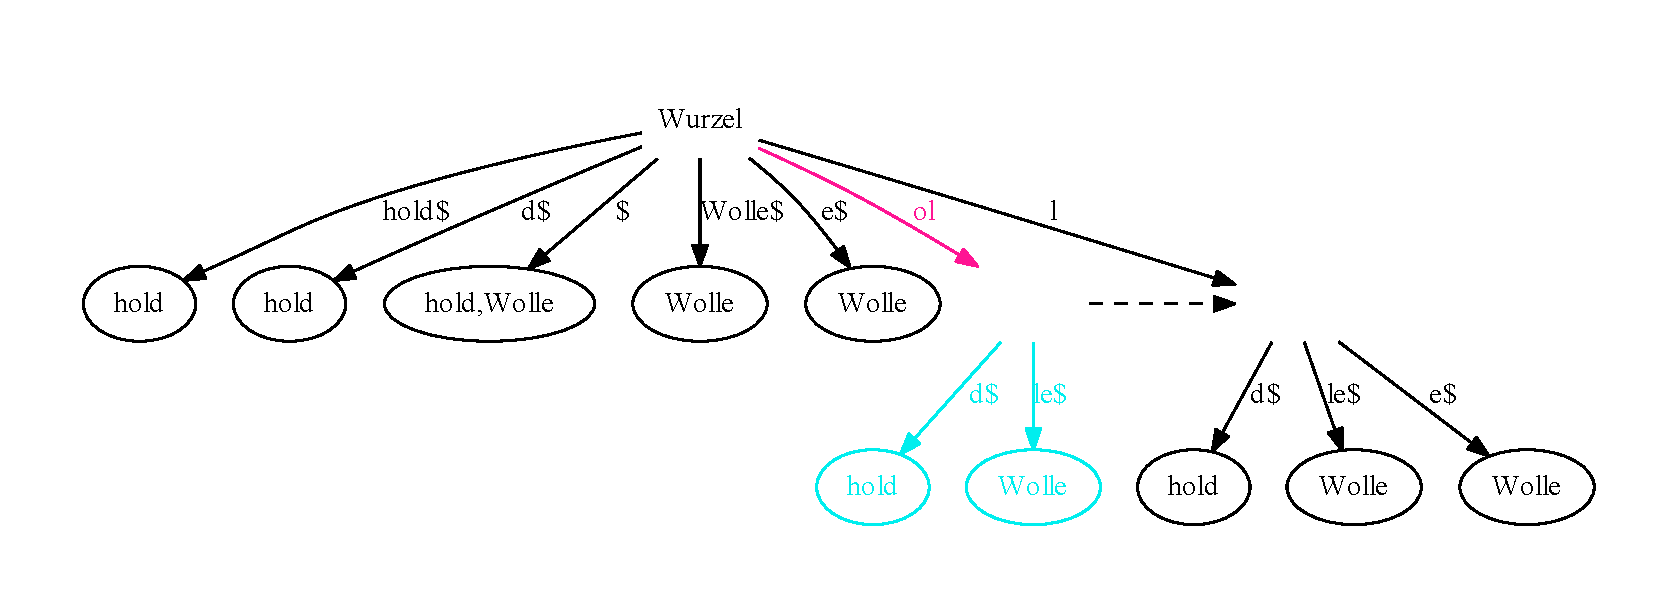
\includegraphics[scale=0.5]{resources/wolleHoldMatchSuffixTree.pdf}
\caption{Teilwortsuche für das Suchmuster \texttt{ol} in einem Beispiel-Suffixbaum für die Worte "`hold"' und "`Wolle"'. Bis zum Ende des pinken Bereichs konnte das Matching erfolgen. Die Suchergebnisse selbst müssen mit Tiefensuche aus dem Suffixbaum geholt werden (in türkis dargestellt).}
\label{fig-matchingSuffixTree}
\end{figure}

\newpage

\subsection{Einfache reguläre Ausdrücke}
\label{algo-regex}

\paragraph{} Wie in Kapitel \ref{algo-pattern-language} bereits angemerkt, wurde für \textit{BiBiServSearch} nur ein eingeschränkter Satz regulärer Ausdrücke implementiert. Dabei war das wesentliche Kriterium bei der Auswahl, dass alle Ausdrücke (bis auf \texttt{*}) je \textit{genau ein} Zeichen matchen. Diese Einschränkung bedeutet zwar eine echte Reduzierung des Funktionsumfangs, ermöglicht aber die Einteilung des Suchmusters in einzelne "`semantische Zeichen"' und vereinfacht dadurch Kompilierung und Suche (siehe auch \ref{arch-pattern}). Daher sind die sonst üblichen Oder-Ausdrücke hier nicht erlaubt (wie z.B. \texttt{(a|ab|abc)}, was bedeuten soll: Entweder $a$ oder $ab$ oder $abc$).
\paragraph{} Der Suchvorgang für reguläre Ausdrücke läuft in folgenden Schritten ab:

\begin{enumerate}
\item Umwandeln des Suchmuster-Strings in einen NEA (siehe auch \ref{meth-automata}).
\item Matching des Automaten gegen den generalisierten Suffixbaum.
\end{enumerate}

\subsubsection{Kompilierung des Suchmusters}

\paragraph{} Wie in Kapitel \ref{arch-pattern} beschrieben geschieht die Kompilierung des Suchmusters mittels eines Transduktors. Dabei wird jedes semantische Zeichen des Suchausdrucks jeweils genau einmal behandelt. Ein semantisches Zeichen eines regulären Ausdrucks kann eine von vier Kategorien haben:
\begin{itemize}
\item Es ist genau ein Zeichen erlaubt (\texttt{ExactPatternChar}), Beispiel: \texttt{a}
\item Es ist irgendein Element aus einer Menge von Zeichen erlaubt \\(\texttt{OneOfPatternChar}), Beispiel: \texttt{[xy]}
\item Es ist irgendein Zeichen erlaubt, das nicht in einer definierten Menge von Zeichen liegt (\texttt{NotOneOfPatternChar}), Beispiel: \texttt{[\^{ }xy]}
\item Es ist irgendein Zeichen erlaubt (\texttt{AnyPatternChar}), Beispiel: \texttt{.}
\end{itemize}
\paragraph{} Unterschieden wird zudem, ob das semantische Zeichen jeweils beliebig oft vorkommen darf oder nicht (ob also ein \texttt{*} folgt oder nicht). Der Kompilierungsalgorithmus ist im Detail als Pseudocode-Algorithmus \ref{code-pattern-compiling} beschrieben.

\begin{algorithm}
\caption{Kompilierung eines Suchmusters}
\label{code-pattern-compiling}
\begin{algorithmic}
\STATE{Initialisiere den momentanen Zustand $z_1$ mit einem leeren Startzustand.}
\STATE{Initialisiere den Stapel $S$ für semantische Zeichen, denen ein \texttt{*} folgt.}
\FORALL{semantische Zeichen $p_1$ des Suchmusters}
	\IF{Auf $p_1$ folgt ein \texttt{*}}
		\IF{Es wurde bereits ein semantisches Zeichen gelesen, dem kein \texttt{*} folgt}
			\STATE{Lege $p_1$ auf $S$.}
		\ENDIF
	\ELSE
		\STATE{Erzeuge einen neuen Zustand $z_2$ des endlichen Automaten.}
		\STATE{Erzeuge eine Kante von $z_1$ nach $z_2$, die mit $p_1$ beschrieben ist.}
		\IF{$S$ ist nicht leer}
			\STATE{Initialisiere die Menge $Z$ als eine Menge von Folgezuständen und Beschriftungen von Kanten, die zu ihnen führen.}
			\STATE{Lege das Tupel $(p_1,z_2)$ in $Z$.}
			\WHILE{$S$ ist nicht leer}
				\STATE{Nimm das oberste semantische Zeichen $p_2$ von $S$ herunter.}
				\IF{$S$ ist leer}
					\STATE{Setze $z_3$ $=$ $z_1$.}
				\ELSE
					\STATE{Erzeuge einen neuen Zustand $z_3$.}
				\ENDIF
				\STATE{Erzeuge eine Kante von $z_3$ nach $z_3$, die mit $p_2$ beschrieben ist.}
				\FORALL{Tupel $(p_3,z_4) \in Z$}
					\STATE{Erzeuge eine Kante von $z_3$ nach $z_4$, die mit $p_3$ beschrieben ist.}
				\ENDFOR
				\STATE{Lege das Tupel $(p_2,z_3)$ in $Z$.}
			\ENDWHILE
		\ENDIF
		\STATE{setze $z_1$ $=$ $z_2$.}
	\ENDIF
\ENDFOR
\STATE{Erzeuge einen akzeptierenden Zustand $f$.}
\STATE{Erzeuge eine Kante von $z_1$ nach $f$, die mit einem Endsymbol beschrieben ist.}
\end{algorithmic}
\end{algorithm}

\paragraph{} Dabei ist folgendes zu beachten:

\begin{itemize}
 \item Im Falle eines Suchmusters ohne reguläre Ausdrücke läuft dieser Algorithmus ohne Besonderheiten durch und betrachtet jedes Zeichen als \\\texttt{ExactPatternChar}.
 \item Für Zeichen, denen ein \texttt{*} folgt, wird ein Stapel/Stack angelegt. Bei der Abarbeitung des Stapels werden für alle Zeichen auf dem Stapel (bis auf das erste) neue Zustände angelegt. Für jeden dieser neuen Zustände müssen Kanten zu jeweils allen noch folgenden Zuständen gezogen werden, weil für jeden \texttt{*}-Ausdruck auch das leere Wort als Match erlaubt ist.
 \item Obwohl das im Pseudocode nicht benannt ist, werden für den Inhalt des Stapels noch Optimierungen durchgeführt: Optimierungen sind möglich, wenn von zwei benachbarten \texttt{*}-Ausdrücken A und B die von A definierte Sprache eine Teilmenge der Sprache von B ist oder umgekehrt (siehe auch \ref{arch-pattern}). Ein Beispiel dafür ist der Ausdruck \texttt{a*.*}. Dieser Ausdruck kann zu \texttt{.*} optimiert werden, weil $\lbrace a\rbrace$ eine Teilmenge des Gesamtalphabets ist.
 \item Da eine Teilwortsuche durchgeführt wird, steht am Beginn und Ende des Musters implizit ein \texttt{.*}. Aus diesem Grunde werden Zeichen, denen zwar ein \texttt{*} folgt, die aber am Beginn oder Ende des Musters stehen, einfach ignoriert.
\end{itemize}

\paragraph{} Das Ergebnis eines Kompilierungsprozesses ist in Abbildung \ref{fig-nea} an einem Beispiel illustriert.

\begin{figure}
\centering
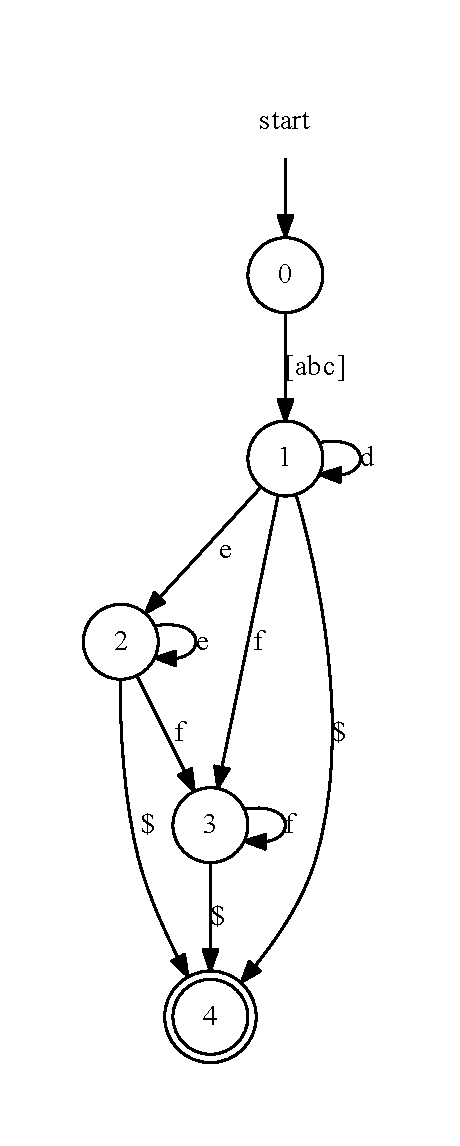
\includegraphics[scale=0.7]{resources/nea.pdf}
\caption{Ein NEA, der dem Suchmuster \texttt{[abc]d*e*f*} entspricht. Der Zustand mit dem "`start"'-Pfeil ist der Startzustand. Der Endzustand ist doppelt umkreist. Das "`\$"'-Zeichen ist ein Endsymbol.}
\label{fig-nea}
\end{figure}

\subsubsection{Matching}

\paragraph{} Der Matchingprozss wird nun über eine Art "`Meta-Automat"' aus dem NEA des Suchmusters und dem Suffixbaum erledigt. Die Zustände des Meta-Automa\-ten sind über die momentane Position im Suffixbaum und den Zustand im NEA charakterisiert. Nur wenn die Kombination aus beidem gleich ist, ist auch das Verhalten des Automaten gleich. Dabei ist zu beachten, dass der Matchingvorgang nicht mehr linear ist sondern indeterministisch mehrere Stränge des Matchings existieren, die über einen Stack künstlich nacheinander ausgeführt werden. Eine Parallelisierung der Ausführungspfade über Threading wäre hier grundsätzlich möglich, ist aber nicht implementiert.
\paragraph{} Diese Vorgehensweise ist analog zur Technik von Baeza-Yates und Gonnet (siehe \cite{baeza-yates}), allerdings in vereinfachter Form, weil hier zu Gunsten einer Beschleunigung der Suchmusterkompilierung NEAs und nicht DEAs implementiert wurden. Auch die bei Baeza-Yates und Gonnet vorgeschlagene binäre Kodierung des Suffixbaums ist hier nicht umgesetzt.
\paragraph{} Das Matching ist im Pseudocode-Algorithmus \ref{code-matching} beschrieben. Wie schon beschrieben kann dann für die Menge der Wort-IDs eine Menge von Vorkommen über den Hauptindex ermittelt werden.

\begin{algorithm}
\caption{Matching-Algorithmus}
\label{code-matching}
\begin{algorithmic}
\STATE{Initialisiere den Stapel der Zustände $S$ und lege den Initialzustand darauf (Wurzel des Baumes und Startzustand des NEA).}
\STATE{Initialisiere die Menge mit Ergebnis-Wort-IDs $W$.}
\WHILE{$S$ ist nicht leer}
	\STATE{Nimm den obersten Zustand $z$ von $S$ herunter.}
	\FORALL{ausgehende Kanten $p$ des NEA-Zustandes in $z$}
		\IF{$p$ ist Endsymbol}
			\STATE{Lege die IDs aller Worte in $W$, die an Blättern notiert sind, die bei einer Tiefensuche im Suffixbaum vom jetzigen Punkt aus zu finden sind.}
		\ELSE
			\IF{momentane Position im Baum ist eine Kante}
				\STATE{Sei $c$ das momentane Zeichen auf der Kante im Baum.}
				\IF{$c$ liegt in der Sprache von $p$}
					\STATE{Erzeuge einen neuen Zustand $z'$ mit der um 1 vorgerückten Baumposition und dem nächsten NEA-Zustand für $p$.}
					\STATE{Lege $z'$ auf $S$.}
				\ENDIF
			\ELSE
				\FORALL{ausgehende Kanten $c$ des momentanen Knotens im Baum, die in der Sprache von $p$ liegen}
					\STATE{Erzeuge einen neuen Zustand $z'$ mit der um 1 vorgerückten Baumposition auf Kante $e$ und dem nächsten NEA-Zustand für $p$.}
					\STATE{Lege $z'$ auf $S$.}
				\ENDFOR
			\ENDIF
		\ENDIF
	\ENDFOR
\ENDWHILE
\end{algorithmic}
\end{algorithm}

\subsection{Inexakte Suche}
\label{algo-inexact}

\paragraph{} Die inexakte Suche ist der komplexeste implementierte Suchmodus. Hier geht es darum, mit heuristischen Mitteln mögliche Tippfehler in Suchanfragen zu korrigieren. Zu diesem Zweck sollen auch \textit{hinreichend ähnliche} Worte als Matches für das Suchmuster zugelassen werden. Wie dieses \textit{hinreichend ähnlich} zu definieren ist steht dabei im Kern des folgenden Abschnitts. Danach wird die Umsetzung dieses Konzeptes besprochen.

\subsubsection{Konzept}

\paragraph{} Ein gängiges heuristisches Modell für die Behandlung von Tippfehlern ist die Betrachtung von Edit-Distanzen, wie sie von Damerau eingeführt wurde (siehe \cite{damerau}, S. 172 und \cite{jurafsky&martin}, S. 145). Die Edit-Distanz beschreibt die Zahl der Arbeitsschritte, die nötig ist, um ein Wort in ein anderes zu überführen. Als ein Arbeitsschritt gilt dabei:

\paragraph{}

\begin{tabularx}{\textwidth}{lX}
\hline
\textbf{Bezeichnung} & \textbf{Beschreibung und Beispiel} \\ [0.1cm]
\hline
insertion &  Weglassen eines Zeichens im Wort (aus "`hold"' wird z.B. "`old"') \\ [0.1cm]
\hline
deletion &  Einfügen eines Zeichens im Wort (aus "`hold"' wird z.B. "`holde"') \\ [0.1cm]
\hline
substitution & Ersetzen eines Zeichens im Wort (aus "`hold"' wird z.B. "`gold"') \\ [0.1cm]
\hline
transposition & Umtausch zweier Zeichen im Wort (aus "`hold"' wird z.B. "`hlod"') \\ [0.1cm]
\hline
\end{tabularx}

\paragraph{} Nach einer Studie von Peterson (siehe \cite{peterson}, S.634) sind etwa 93-94 \% der Tippfehler nur einen Arbeitsschritt vom eigentlich gemeinten Wort entfernt. Daher konzentriert sich die inexakte Suche hier darauf, genau diese Fehler mit Edit-Distanz 1 zu beheben.
\paragraph{} Die Idee ist dabei wie folgt: Versuche, das Suchwort wie in den vorherigen Kapiteln im Baum zu finden (siehe vor allem \ref{algo-regex}). Sobald ein Buchstabe im Suchwort nicht mehr mit dem Buchstaben im Baum übereinstimmt, versuche den Fehler zu beheben, in dem, falls möglich, jeder der obigen Arbeitsschritte angewendet wird. Bei einem erneuten Fehler wird der Suchvorgang abgebrochen.
\paragraph{} Dieser Algorithmus verzichtet dabei auf die Ansätze des dynamic programming, wie es bei Cobbs, Ukkonen und Jokinen Anwendung findet (siehe \cite{approxTreesUkkonen1, approxTreesUkkonen2,approxTreesCobbs}). Diese Vereinfachung ist nur deshalb zulässig, weil die maximale Edit-Distanz in der vorliegenden Implementierung 1 beträgt. Andernfalls könnte es passieren, dass durch mehrfache Anwendung von Edit-Operationen Zustände wiederholt werden und dadurch eine erheblich schlechtere worst-case-Laufzeit erzielt wird. Wegen der Vereinfachung ist es auch nicht nötig, eine von den o.g. Autoren vorgeschlagene Tabelle mit Edit-Operationen explizit aufzubauen. Diese wird mithin implizit über die \texttt{MatchingStates} kodiert.

\subsubsection{Umsetzung}

\paragraph{} Dass \textit{alle} Arbeitsschritte zur Fehlerkorrektur angewendet werden bedeutet, dass der Matchingvorgang indeterministisch wird. Da das bestehende System mit \texttt{MatchingStates} für reguläre Ausdrücke aber bereits in der Lage ist, Indeterminismus zu behandeln, liegt es nahe, einfach dieses System zu erweitern.
\paragraph{} Ein Zustand des dort besprochenen "`Meta-Automaten"' erhält also ein weiteres Charakteristikum: Ist die Anwendung eines Arbeitsschrittes noch erlaubt oder nicht (Bei einer Teilwortsuche, die kein inexaktes Matching erlaubt, wird dies schon im Initialzustand auf "`nein"' gesetzt)? Beim ersten mismatch wird versucht, den Fehler durch die Anwendung der beschriebenen Arbeitsschritte zu beheben. Beim neu entstehenden Zustand wird dann die Frage, ob die Anwendung eines Arbeitsschrittes erlaubt ist, mit "`nein"' beantwortet. So wird erreicht, dass alle Fehler mit einer Edit-Distanz von 1 behoben werden. Dank des Konzeptes des Meta-Automaten geschieht dies aber nur, wenn auch wirklich ein mismatch auftritt. Gegenüber der naiven Implementierung, einfach blind alle Permutationen des Suchmusters mit Edit-Distanz 1 zu erzeugen (klassische "`Neighborhood generation"' wie in \cite{approximateIndexing} beschrieben) und danach jeweils zu suchen, ist dieses Vorgehen also eine deutliche Verbesserung.
\paragraph{} Der für die Arbeitsschritte jeweils neue Zustand des Meta-Automaten wird wie folgt berechnet:

\paragraph{}

\begin{tabularx}{\textwidth}{lX}
\hline
\textbf{Bezeichnung} & \textbf{Neuer Zustand} \\ [0.1cm]
\hline
insertion & Rücke im Suffixbaum um einen Schritt vor. \\ [0.1cm]
\hline
deletion & Rücke im NEA zum nächsten Zustand vor. \\ [0.1cm]
\hline
substitution & Rücke sowohl im Suffixbaum als auch im NEA um einen Schritt vor. \\ [0.1cm]
\hline
transposition & Siehe unten. \\ [0.1cm]
\hline
\end{tabularx}

\paragraph{} Diese Operationen sind bis auf transpositions trivial umsetzbar. Transpositions werden wie in Algorithmus \ref{code-swap} beschrieben behandelt.

\begin{algorithm}
\caption{Transposition-Algorithmus}
\label{code-swap}
\begin{algorithmic}
\STATE{Sei $c$ das momentane Zeichen im Suffixbaum und $z_0$ der momentane Zustand des NEA.}
\FORALL{ausgehende Kanten $p_0$ von $z_0$}
\STATE{Sei $z_1$ der Folgezustand für $p_0$.}
\IF{$z_1$ $\neq$ $z_0$}
\FORALL{ausgehende Kanten $p_1$ von $z_1$, die $c$ akzeptieren}
\STATE{Sei $z_2$ der Folgezustand für $p_1$.}
\STATE{Erzeuge einen neuen NEA-Zustand $z_3$.}
\STATE{Erzeuge eine Kante von $z_3$ über $p_1$ nach $z_2$.}
\STATE{Setze $z_3$ als neuen NEA-Zustand. Die Position im Suffixbaum bleibt unverändert.}
\ENDFOR
\ENDIF
\ENDFOR
\end{algorithmic}
\end{algorithm}

\paragraph{} Über die Erzeugung des virtuellen NEA-Zustandes $z_3$ wird sicher gestellt, dass der NEA genau dann in den Zustand $z_2$ übergeht, wenn zwei Zeichen im Suchwort in genau umgekehrter Reihenfolge im Baum vorkommen. Das entspricht exakt dem, was man mit einer transposition erreichen wollte.
\paragraph{} Zudem ist über diesen Mechanismus das inexakte Matching mit regulären Ausdrücken kompatibel\footnote{Allerdings wird verhindert, dass \texttt{*}-Ausdrücke bei der Fehlerbehebung in Betracht gezogen werden. Edit-Operationen auf diesen Ausdrücken würden beispielsweise dazu führen, dass bei Anwendung der deletion-Regel im NEA auf den gleichen Zustand vorgerückt wird, sich also am Zustand eigentlich nichts ändert, das System aber trotzdem damit umgeht als sei hier eine Edit-Operation angewandt worden. Das könnte zu verwirrenden Ergebnissen für Nutzende führen.}.

\subsection{Bewertung der Suchergebnisse}
\label{algo-scoring}

\paragraph{} Nachdem eine Menge von Vorkommen der Ergebnisworte erstellt worden ist, ist der letzte Schritt die Umsetzung dieser Menge von Vorkommen in eine sortierte Liste von Dokumenten-Identifikatoren (siehe auch \ref{arch-docIndex}), die Nutzenden auf ihre jeweilige Suchanfrage hin zurückgegeben werden kann.
\paragraph{} Wie im Konzept vorgeschlagen (siehe \ref{meth-scoring}) erfolgt die Sortierung der Dokumente nach einem zweistufigen \texttt{SearchScore}:
\begin{enumerate}
\item Wie viele Vorkommen von Matches enthält das Dokument? (primärer Score)
\item Wie weit sind die Matches vom ursprünglichen Suchmuster entfernt? (sekundärer Score)
\end{enumerate}

\paragraph{} Dabei wird vornehmlich nach dem primären Score sortiert und erst bei gleichem Wert der sekundäre Score in Betracht gezogen. Das heißt: Dokumente, die mehr Treffer enthalten, werden auch als erstes genannt. Dokumente, die gleich viele Treffer enthalten, werden dann zuerst genannt, wenn die Treffer im Durchschnitt besser dem Suchmuster entsprechen.
\paragraph{} Der Prozess ist im Pseudocode-Algorithmus \ref{code-scoring} beschrieben.

\begin{algorithm}
\caption{Bewertungsalgorithmus für Suchergebnisse}
\label{code-scoring}
\begin{algorithmic}
\STATE{Initialisiere eine HashMap $H$, die Dokumente auf ihren \texttt{SearchScore} abbildet.}
\FORALL{Vorkommen $v$ in der Menge der Ergebnisvorkommen}
	\STATE{Sei $d$ das Dokument, das $v$ enthält.}
	\IF{$d$ ist in $H$ enthalten}
		\STATE{Sei $S$ das Score-Objekt für $d$.}
		\STATE{Erhöhe den Primärscore in $S$ um 1.}
		\STATE{Berechne den Sekundärscore $s'$ für v.}
		\STATE{Erhöhe den Sekundärscore in $S$ um $s'$.}
	\ELSE
		\STATE{Erstelle ein neues Score-Objekt $S$.}
		\STATE{Setze den Primärscore auf 1.}
		\STATE{Berechne den Sekundärscore $s'$ für v.}
		\STATE{Setze den Sekundärscore in $S$ auf $s'$}
	\ENDIF
	\STATE{Schreibe $S$ für $d$ in $H$.}
\ENDFOR
\end{algorithmic}
\end{algorithm}

\paragraph{} Die Berechnung des Sekundärscores unterscheidet sich dabei je nach Suchmodus. Generell gilt: Ein höherer Sekundärscore bedeutet eine größere Entfernung vom Suchmuster. Bei exakter Suche ist dieser Score immer 0 (weil ja \textit{per definitionem} Matches dem Suchmuster exakt entsprechen müssen). Bei der Teilwortsuche wird die Länge des Matches mit der Länge des gematchten Teilwortes verglichen. Die Differenz beider Längen ist der Sekundärscore. Bei der inexakten Suche erfolgt die Berechnung auf die gleiche Weise, es wird aber noch der Wert 3 addiert, falls Methoden der inexakten Suche benutzt werden mussten, um dieses Match zu finden.

\paragraph{} Zusätzlich wird für jedes Ergebnisvorkommen der \textit{Kontext} bestimmt, das heißt: Ausgehend vom Wort, das gematcht wurde, werden die vorherigen drei Worte und die nachfolgenden drei Worte bestimmt, um Nutzenden des Programms mehr Komfort zu bieten. Dies ist über die Referenzierung von Vorgängern und Nachfolgern bei Vorkommen möglich (siehe auch \ref{arch-index}).

\newpage

\subsection{Entfernen eines Dokuments}
\label{algo-removeDoc}

\paragraph{} Wenn ein Dokument aus dem Suchraum entfernt werden soll, wird das Dokument und sein Inhalt aus allen Indizes entfernt. Zuerst wird für eine gegebene URL die Dokumenten-ID aus dem Dokumentenindex herausgesucht. Mit dieser ID kann über den Hauptindex iteriert und es können alle Vorkommen entfernt werden, die auf diese ID verweisen. Zusätzlich wird bei dieser Gelegenheit auch geprüft, ob die Menge von Vorkommen, auf die eine Wort-ID im Hauptindex verweist, leer geworden ist. Falls ja wird der Eintrag dieses Wortes ganz aus Haupt- und Wortindex entfernt.
\paragraph{} Problematisch dabei ist, dass die Worte nicht aus dem Suffixbaum entfernt werden können (siehe auch \ref{meth-addAndRemove}). Auf die Suchergebnisse hat das keinen Einfluss, denn im Hauptindex wird dann für die fragliche Wort-ID schlicht kein Verweis auf die gelöschten Dokumente gefunden. Dennoch führt das langfristig dazu, dass der Suffixbaum mit Einträgen, die zu keinem Ergebnis mehr führen, überfüllt wird. Das kostet Speicher und Rechenzeit beim Suchen.
\paragraph{} Wie im Konzept beschrieben (siehe \ref{meth-addAndRemove}), wurden zwei Mechanismen eingeführt, um dieses Problem zu entschärfen:
\begin{enumerate}
 \item Von außen kann bei Bedarf die Funktion \texttt{rebuildTree} der Klasse \texttt{WordIndex} aufgerufen werden. Bei einem Aufruf wird der Suffixbaum neu aus dem momentanen Wortindex aufgebaut. Dabei werden  gelöschte Einträge nicht mehr mit in den neuen Baum übernommen und der alte Baum wird aus dem Speicher gelöscht.
 \item Beim Neueinfügen von Dokumenten in den Baum wird der Baum ebenfalls neu aufgebaut (siehe auch \ref{arch-session}). Auch dabei werden alle gelöschten Einträge nicht mehr in den neuen Baum übernommen.
\end{enumerate}


\chapter{Ergebnisse}
\label{fazit}

\paragraph{} Abschließend bleibt nun noch auszuwerten, wie effizient die implementierten Lösungen sind (siehe \ref{fazit-complexity}) und ob die gestellten Anforderungen erfüllt wurden (siehe \ref{fazit-evaluation}). Außerdem sind in Abschnitt \ref{fazit-ausblick} noch Ansätze dokumentiert, mit denen \textit{BiBiServSearch} weiter verbessert werden kann.

\section{Komplexität}
\label{fazit-complexity}

\paragraph{} Die Komplexität der implementierten Algorithmen wird für drei Fälle betrachtet: Das Einfügen von Dokumenten in den Suchraum (siehe \ref{compl-insert}), die Suche selbst (siehe \ref{compl-search}) und schließlich das Entfernen von Dokumenten aus dem Suchraum (siehe \ref{compl-remove}). %Außerdem sind die Ergebnisse noch einmal in Kürze in einer tabellarischen Übersicht zusammengefasst (siehe \ref{compl-table}).
\paragraph{} Die Analyse erfolgt so weit möglich nicht nur theoretisch sondern auch empirisch. Praktische Laufzeit- und Speicherverbrauchsanalysen wurden dabei mit Hilfe von NetBeans\texttrademark Profiling vorgenommen (die entsprechende Konfiguration kann in Anhang \ref{profiling} nachgelesen werden).
\paragraph{} Die empirischen Testdaten waren eine Mischung aus 76 Dateien verschiedener Formate (XML, PDF und einfacher Text) in Deutsch und Englisch mit einer Dateigröße von insgesamt 257 MB, 104441 verschiedenen Worten und einer Textlänge von 369325 Worten.

\subsection{Einfügen von Dokumenten}
\label{compl-insert}

\paragraph{} Wie bereits in \ref{algo-addDoc} beschrieben erfolgt das Einfügen von Dokumenten in den Suchraum in zwei Schritten: Zuerst werden die Worte in Hash-Tabellen eingefügt und dann im Suchraum indiziert.
\paragraph{} Das Einfügen von Einträgen in die Hash-Tabellen hat die Laufzeit $\mathcal{O}(1)$. Insgesamt müssen dabei für $d$ Dokumente mit $v$ Vorkommen von $w$ Worten $\mathcal{O}(d + w + v)$ Einträge gemacht werden. Lediglich das Einlesen des Dokumenteninhalts und die Vorverarbeitung der Worte hat die Laufzeit $\mathcal{O}(n_{neu})$, wobei $n_{neu}$ die Länge des neu eingefügten Textinhalts in Zeichen ist.
\paragraph{} Die Laufzeitklasse wird auch durch das Einfügen in den Suffixbaum grundsätzlich nicht verändert, weil Ukkonnens Algorithmus in linearer Zeit läuft (siehe \cite{gusfield}, S. 94).
\paragraph{} Allerdings wird durch den Neuaufbau des Suffixbaumes vor der Einfügung des neuen Inhalts die Laufzeit deutlich verschlechtert, weil hier der gesamte alte Wortinhalt erneut berücksichtigt wird. Die Laufzeit erhöht sich also auf $\mathcal{O}(w_{alt} + n_{neu})$\footnote{Es ist allerdings implementiert, dass die Laufzeit sich nicht weiter verschlechtert, wenn mehrere Dokumente eingefügt werden. Es wird nur einmal, vor dem ersten Dokument, der Baum neu aufgebaut und ab dann mit der Baumkopie weiter gearbeitet, bis alle Dokumente eingefügt sind (siehe auch Session-System in \ref{arch-session}).}. Das zeigt sich auch im Praxistest (siehe Abbildung \ref{fig-insert}).

\graph{resources/graph_insert.pdf}{fig-insert}{Laufzeit (in Millisekunden) für die Einfügung von Dokumenten in den Suchraum abhängig von der indizierten Textlänge in Worten. Wie in Kapitel \ref{compl-insert} beschrieben ist hier eine lineare Abhängigkeit von der indizierten Textlänge in Zeichen zu erwarten. Leichte Abweichungen von einer Geraden im Graphen sind also durch eine variierende durchschnittliche Wortlänge zu erklären.}

\paragraph{} Die Speicherkomplexität ist ganz ähnlich, allerdings mit ein paar Besonderheiten: Suffixbaum und Wortindex sind lediglich von der Länge aller unterschiedlichen Worte des Suchraums abhängig, nicht aber von der Textlänge insgesamt. Für die worst case-Komplexität spielt das zwar keine Rolle, in der Praxis wiederholen sich Worte allerdings häufig und es ist in der Regel zu erwarten, dass die Anzahl der Wiederholungen mit größerer Textlänge ansteigt (siehe Abbildung \ref{fig-wordsToOccs}).

\graph{resources/graph_words-occs.pdf}{fig-wordsToOccs}{Durchschnittliche Anzahl von Vorkommen pro Wort abhängig von der indizierten Textlänge in Worten.}

\paragraph{} Der Dokumentenindex ist noch kleiner und lediglich von der Anzahl der Dokumente abhängig (im worst case ist die Dokumentenanzahl allerdings auch durch die Textlänge beschränkt).
\paragraph{} Am größten bleibt der Hauptindex, der tatsächlich alle Vorkommen von Worten enthält. Insgesamt liegt die Speicherkomplexität demnach ebenfalls bei $\mathcal{O}(w + d + v)$. Diese Erwartung bestätigt sich im Praxistest: Mit wenigen Ausnahmen scheint sogar eine lineare Abhängigkeit von der Anzahl indizierter Worte, nicht von deren Vorkommen vorzuliegen (siehe Abbildung \ref{fig-storage-occs} bzw. Abbildung \ref{fig-storage-words}).

\graph{resources/graph_storage-occs.pdf}{fig-storage-occs}{Speicherverbrauch der Anwendung (in Kilobyte) abhängig von der indizierten Textlänge in Worten.}

\graph{resources/graph_storage-words.pdf}{fig-storage-words}{Speicherverbrauch der Anwendung (in Kilobyte) abhängig von der Anzahl unterschiedlicher indizierter Worte.}

\paragraph{} Anzumerken bleibt, dass diese Berechnungen sich nur auf den Code beziehen, der zu \textit{BiBiServSearch} selbst gehört. Nicht mit einbezogen ist der Code des "`Apache Tika"'-Pakets. Die praktische Laufzeit ist durch dieses Paket schlechter. Eine genaue Analyse der Laufzeit dieses Pakets war nicht möglich, weil die Laufzeit hier offenbar von der Art des Dateiformats abhängt (das Öffnen von PDFs ist anscheinend besonders aufwändig). In einer groben Abschätzung aber kann davon ausgegangen werden, das hier wie bei der Vorverarbeitung eine lineare Abhängigkeit von der Textlänge vorliegt (siehe auch Abbildung \ref{fig-parsing}).

\graph{resources/graph_parsing.pdf}{fig-parsing}{Laufzeit (in Millisekunden) für das Parsen von Dokumenten durch das "`Apache Tika"'-Paket abhängig von der indizierten Textlänge in Worten.}

\subsection{Suche}
\label{compl-search}

\paragraph{} Bei der Komplexitätsberechnung für Suchanfragen ist zu beachten, dass sie in zwei Schritten abläuft: Zuerst wird die Suchanfrage bearbeitet und dann die Ergebnisse sortiert. Die Laufzeit ist die Summe beider Prozesse.
\paragraph{} In den allermeisten Fällen blieben die Antwortzeiten bei praktischer Messung der Laufzeit selbst bei großen Suchräumen sehr klein (unter 100 Millisekunden). Sollte dort ein Zusammenhang mit der Textlänge vorliegen ließ er sich nicht messen. Die kurzen Antwortzeiten werden im Folgenden als Beleg dafür betrachtet, dass im average case die Antwortzeit nicht von der indizierten Textlänge abhängt.

\subsubsection{Exakte Suche}

\paragraph{} Die Komplexität lässt sich am einfachsten für Suchanfragen mit nur einem Wort bestimmen: In diesem Fall muss für das Wort nur dessen ID im Wort-Index und für die Wort-ID die Vorkommen im Haupt-Index abgefragt werden. Die Komplexität für Zugriffe auf Hash-Tabellen ist $\mathcal{O}(1)$ (siehe \cite{knuth}, S. 538). Anders sieht es allerdings für exakte Suchanfragen mit mehreren Worten aus: Hier muss für alle Vorkommen des ersten Wortes geprüft werden, ob alle übrigen Worte der Suchanfrage auch tatsächlich in der richtigen Reihenfolge vorliegen. Die Laufzeit ist also 

\paragraph{} $\mathcal{O}\left(\sum_{i \in V(w_1)} \left( 1 + \sum_{j=2}^m \prod_{k=2}^j \delta(w_k,w(i+k)) \right)\right)$,

\paragraph{} wobei $w_1, \dots, w_m$ die Worte der Suchanfrage sind, $V(w_1)$ die Positionen der Vorkommen für das erste Suchwort im Text meint, $w(n)$ mit $n \in \mathbb{N}$ das Wort im Text an Stelle $n$ und schließlich $\delta(w_i,w_j)$ für die Worte $w_i$ und $w_j$ definiert ist als $1$, falls $w_i = w_j$ und $0$ sonst.
\paragraph{} Im worst case kann $\delta(w_i,w_j)$ immer $1$ sein, wenn alle Vorkommen des ersten Wortes des Suchmusters auch tatsächlich valide Ergebnisvorkommen sind. Also beträgt die worst case-Laufzeit $\mathcal{O}(m \cdot V(w_1))$.

\subsubsection{Teilwortsuche}

\paragraph{} Sofern das Suchmuster einer Teilwortsuche ein Suffix eines indizierten Wortes ist, ist die Frage nach der Komplexität einfach zu beantworten: Für jedes Suffix eines existierenden Wortes existiert ein eindeutiger Pfad im Suffixbaum. Dieser muss nur besucht werden. Die dafür nötige Zeit ist $\mathcal{O}(m)$, wobei $m$ die Länge des Suchmusters ist.
\paragraph{} Komplizierter wird es allerdings, wenn das Suchmuster ein echtes Teilwort ist. In so einem Fall müssen nach dem Ende des Matchings selbst mit einer Tiefensuche alle folgenden Blätter besucht und die dort eingetragenen Wort-IDs zusammengetragen werden (siehe auch Algorithmus \ref{code-matching}). Der Vorteil ist, dass hier der Inhalt der Kanten des Baumes nicht mehr angesehen werden muss. Wir dürfen einfach durch alle Knoten springen, bis alle Blätter gefunden sind. Die Laufzeit ist also nur von der Anzahl der Knoten abhängig. Für die Knoten gilt: Es wird nur ein interner Knoten erzeugt, wenn ein Split durchgeführt werden muss. Das wiederum geschieht entweder dann, wenn von einem gegebenen Punkt im Baum ein neues Wort anders endet als ein bisheriges oder wenn ein anderes Suffix eines Wortes anders endet\footnote{Ein triviales Beispiel für diesen Fall ist das Wort \texttt{aaa\$}. Hier werden zwei Splits durchgeführt, weil die verschiedenen Suffixe unterschiedlich enden.}. Dementsprechend ist die Anzahl der Knoten abhängig von der Anzahl der Positionen, an denen das Muster die Matches matcht. Das ist im schlimmsten Fall an jeder Position der Matches der Fall. Die Laufzeit ist dementsprechend $\mathcal{O}(m + |w|)$, wobei $|w|$ die summierte Länge aller Ergebnisworte meint (das ist analog zur Beschreibung von Gusfield; siehe \cite{gusfield}, S. 122).

\subsubsection{Reguläre Ausdrücke}

\paragraph{} Noch komplizierter wird es, sobald reguläre Ausdrücke im Suchmuster auftreten. In diesem Fall lässt sich die Anzahl der benötigten Rechenschritten nicht mehr auf eine einfache Formel bringen: Es ist immer entscheidend, an welcher Stelle im Baum das Matching gerade ist und wie viele der verfügbaren Zeichen im Baum vom momentanen Zustand des NEA akzeptiert werden. Es entsteht also eine rekursive Gleichung:
\paragraph{} $r(z_i,\alpha_i)$ $=$ $1$ $+$ 
$\sum_{p_{i+1} \in P(z_i)}$ 
$\sum_{c_{i+1} \in M(p_{i+1}, \alpha_i)}$ 
$ r\left(z_{i+1}(z_i,p_{i+1}),\alpha_{i+1}(\alpha_i,c_{i+1})\right)$ und $r(z_{m'},\alpha_{m'}) = 1$,
\paragraph{}wobei gilt:
\begin{itemize}
 \item $r(z_i,\alpha_i)$ ist die Anzahl der Rechenschritte, die im Schritt $i$ noch nötig sind.
 \item ${m'}$ ist hier \underline{nicht} die Länge des Suchmusters, sondern die Anzahl der Schritte des Matching-Algorithmus. Dass sich das unterscheiden kann wird am Beispiel \texttt{a*} klar: Hier kann der Matching-Prozess beliebig viele Schritte brauchen.
 \item $\alpha_i$ $:=$ Position im Baum im Schritt $i$.
 \item $z_i$ $:=$ Zustand des NEA im Schritt $i$.
 \item $c_{i+1}$ $:=$ Zeichen im Baum, das zum Schritt $i+1$ führt.
 \item $p_{i+1}$ $:=$ \texttt{PatternChar} bzw. Ausdruck auf einer Kante im NEA, der zum Schritt $i+1$ führt.
 \item $\alpha_{i+1}(\alpha_i,c_{i+1})$ $:=$ Position im Baum im Schritt $i+1$, wenn die Position im Baum in Schritt $i$ $\alpha_i$ war und man sich im Baum entlang des Zeichens $c_{i+1}$ weiterbewegt.
 \item $z_{i+1}(z_i,p_{i+1})$ $:=$ Zustand des NEA im Schritt $i+1$, wenn der Zustand im Schritt $i$ $z_i$ war und man sich entlang der Kante mit dem Ausdruck $p_{i+1}$ weiterbewegt.
 \item $P(z_i)$ $:=$ Alle ausgehenden Kantenausdrücke für $z_i$.
 \item $M(p_{i+1},\alpha_i)$ $:=$ Alle ausgehenden nächsten Buchstaben für $\alpha_i$, die vom Ausdruck $p_{i+1}$ akzeptiert werden.
\end{itemize}

\paragraph{} Die Laufzeit für die Suche insgesamt entspricht dann $r(z_0,\alpha_0)$, wobei $z_0$ der Initialzustand des Automaten und $\alpha_0$ die Wurzel des Suffixbaums ist.
\paragraph{} Dabei ist im Allgemeinen die Anzahl der Elemente für $P(z_i)$ durch die Länge des Suchmusters $m$ beschränkt. Hier ist der worst case ein Muster des Typs \texttt{a*b*c*d* $\dots$}, weil in diesem Fall vom ersten Zustand aus für alle folgenden Zeichen des Musters eine ausgehende Kante zum Finalzustand existieren muss (siehe auch \ref{algo-regex}). Für die Anzahl der Elemente von $M(p_{i+1},\alpha_i)$ ist hingegen der worst case der Ausdruck \texttt{.*} \footnote{Tatsächlich ist dieser Spezialfall explizit im Code untersagt. Allerdings lassen sich trivial Fälle konstruieren, in denen ähnliche Ausdrücke mit bestimmten Bäumen eine gleiche Laufzeit erzeugen.}, weil dann für jeden Knoten im Baum alle ausgehenden Kanten bearbeitet werden müssen. Die obere Schranke für die ausgehenden Kanten ist $|A|$, also die Größe des Alphabets.
\paragraph{} Die beiden worst cases sind allerdings inkompatibel, weil bei der vorliegenden Implementierung des Algorithmus in der Vorverarbeitung von Suchmustern der Ausdruck \texttt{.*.*.* $\dots$} zu \texttt{.*} optimiert wird (siehe auch \ref{algo-regex}) und demnach die Anzahl für $P(z_i)$ in jedem Rechenschritt auf 1 absinkt. Es folgt also für die Laufzeit:

\paragraph{} $r(z_i,\alpha_i)$ $=$ $1 + |A| \cdot r(z_{i+1},\alpha_{i+1})$ $\Rightarrow$ $r(z_0,\alpha_0) = \sum_{i=0}^{m'} |A|^i$ $\Rightarrow$ $\mathcal{O}(|A|^{m'})$

\paragraph{} oder:

\paragraph{} $r(z_i,\alpha_i)$ $=$ $1 + |m| \cdot r(z_{i+1},\alpha_{i+1})$ $\Rightarrow$ $r(z_0,\alpha_0) = \sum_{i=0}^{m'} m^i$ $\Rightarrow$ $\mathcal{O}(m^{m'})$

\paragraph{} Dabei ist ${m'}$ durch die Länge des längsten indizierten Wortes beschränkt. Ebenfalls beschränkt ist die Anzahl der nötigen Rechenschritte für die Suche durch die Summe aller indizierten Wortlängen. Noch genauer ist die Laufzeit also: $\mathcal{O}(min \lbrace \left(max \lbrace m, |A| \rbrace \right)^{m'} , |w| \rbrace)$. In der Tat deutet sich dieser lineare Zusammenhang mit der Anzahl indizierter Worte auch in der Praxis an (siehe Abbildung \ref{fig-graph-regex}).

\graph{resources/graph_regex.pdf}{fig-graph-regex}{Laufzeit (in Millisekunden) für eine Suche mit regulären Ausdrücken abhängig von der Anzahl unterschiedlicher indizierter Worte. Suchmuster war hier \texttt{![abc][\^{}z]*[abc]!}.}

\paragraph{} Bei Berücksichtigung der Laufzeit für die Kompilierung kommt noch ein Summand $\mathcal{O}(m^2)$ hinzu, weil im worst case für alle Zustände alle jeweils nachfolgenden Zustände berücksichtigt werden müssen (das ist z.B. beim Suchmuster \texttt{ab*c*d*e} der Fall, siehe auch Algorithmus \ref{code-pattern-compiling}).

\subsubsection{Inexakte Suche}

\paragraph{} Bei der inexakten Suche werden zusätzlich zum ursprünglichen Suchmuster alle Varianten gesucht, die bei einer Edit-Distanz von 1 aus dem Suchmuster entstehen (siehe \ref{algo-inexact}). Zwar werden hier durch die Konstruktion des Algorithmus nur solche Varianten benutzt, die auch tatsächlich im Suffixbaum auftreten, aber im schlimmsten Fall müssen tatsächlich alle gesucht werden. Dabei setzt sich die Anzahl der Varianten wie folgt zusammen (im folgenden ist $m$ die Länge des Suchmusters und $|A|$ die Größe des Alphabets):

\paragraph{}

\begin{tabularx}{\textwidth}{lX}
\hline
\textbf{Bezeichnung} & \textbf{Anzahl der Varianten} \\ [0.1cm]
\hline
insertion & An $m+1$ Positionen können je $|A|$ Zeichen eingefügt werden. Das macht insgesamt $|A| \cdot (m+1)$ Varianten.\\ [0.1cm]
\hline
deletion & Bei einer Länge des Suchmusters von $m$ kann nur an $m$ Stellen ein Zeichen entfernt werden, also $m$ Varianten. \\ [0.1cm]
\hline
substitution & An $m$ Positionen kann ein Zeichen des Suchmusters durch je $|A|-1$ andere ersetzt werden, also existieren hierfür $m \cdot (|A|-1)$ Varianten. \\ [0.1cm]
\hline
transposition & An $m-1$ Positionen (nicht an der letzten) kann ein Zeichen mit dem folgenden Zeichen vertauscht werden, also kommen noch einmal $m-1$ Varianten hinzu. \\ [0.1cm]
\hline
\end{tabularx}

\paragraph{} Insgesamt entsteht so eine Anzahl von $2 \cdot |A| \cdot m + |A| + m -1$ Varianten (siehe auch \cite{peterson}, S. 635) und eine Laufzeit von $\mathcal{O}(|A| \cdot m \cdot t_{Suche})$, wobei $t_{Suche}$ die Zeit für die Suche nach dem Wort im Suffixbaum ist. Im "`normalen"' Fall ohne reguläre Ausdrücke wäre die worst case-Laufzeit demnach $\mathcal{O}(|A| \cdot m^2 )$.

\subsubsection{Bewertung von Suchergebnissen}

\paragraph{} Bei der Bewertung eines Dokuments muss jedes der $k$ Ergebnisvorkommen, das gefunden wurde, noch einmal angeschaut werden. Wie im Pseudocode-Algorithmus \ref{code-scoring} zu sehen wird dabei nur einmal über die Menge der Vorkommen iteriert. Die Ergebnisliste von Dokumenten muss dann noch einmal abhängig vom Score sortiert werden. Die Sortierung hat gemäß Java\texttrademark-Dokumentation (siehe \cite{javaCollectionSort}) eine worst case-Laufzeit von $\mathcal{O}(d \cdot log(d))$, wobei $d$ hier die Anzahl der Ergebnisdokumente ist. Das Heraussuchen des Kontextes geschieht dank der Implementierung der Vorkommen als doppelt verketteter Liste in konstanter Laufzeit. Insgesamt ergibt sich für die Bewertung der Suchergebnisse also eine Laufzeit von $\mathcal{O}(k + d \cdot log(d))$. Dabei ist $d$ im Allgemeinen sehr viel kleiner als $k$.

\subsection{Entfernen von Dokumenten}
\label{compl-remove}

\paragraph{} Die verschiedenen Indizes der Anwendung sind darauf ausgelegt, für eine Wort-ID Vorkommen, für Vorkommen Dokumente und für Dokumente deren URLs zu finden - der umgekehrte Weg ist weniger einfach. Tatsächlich müssen Dokumenten- und Hauptindex, wie in Abschnitt \ref{algo-removeDoc} bereits angedeutet, iterativ durchlaufen werden, um erst für die gegebene URL eine Dokumenten-ID und dann für die Dokumenten-ID alle Vorkommen zu finden. Allerdings müssen die Vorkommen selbst nicht durchlaufen werden: Vorkommensmengen (Klasse \texttt{OccurenceSet}) sind als \texttt{HashMap} implementiert, in denen wiederum Mengen von Vorkommen abhängig von Dokumenten-IDs abgespeichert werden. Es muss also nur über die Schlüssel, nicht über die Werte des Haupt-Index iteriert werden. Das verbessert die Laufzeit auf $\mathcal{O}(d + w)$, wobei $d$ die Anzahl der indizierten Dokumente und $w$ die Anzahl der unterschiedlichen, indizierten Worte ist.
\paragraph{} Im Praxistest lässt sich die Laufzeit nur schwer messen, weil eine einzelne Entfernen-Operation außer bei unrealistisch großen Dokumenten relativ schnell abgeschlossen ist. Deshalb wurde für den Test über alle indizierten Dokumente iteriert. Dementsprechend ist die erwartete Laufzeit $\Theta(d^2 + d \cdot w)$ bzw. $\Theta(d \cdot w)$, weil in der Praxis $d$ deutlich kleiner als $w$ ist. Das deckt sich auch mit den tatsächlichen Ergebnissen (siehe auch \ref{fig-remove}).

\graph{resources/graph_remove}{fig-remove}{Laufzeit (in Millisekunden) für die Entfernung \underline{aller} indizierten Dokumente in Millisekunden abhängig vom Produkt aus der Anzahl indizierter Dokumente und Worte.}

% \subsection{Tabellarische Übersicht}
% \label{compl-table}
% 
% \paragraph{} Als Syntax gilt hier:
% 
% \paragraph{}
% 
% \begin{tabularx}{\textwidth}{lX}
% \hline
% \textbf{Buchstabe} & \textbf{Bedeutung}\\ [0.1cm]
% \hline
% $d$ & Anzahl der Dokumente\\ [0.1cm]
% \hline
% $n$ & Anzahl der Zeichen bzw. der Textlänge in Zeichen \\ [0.1cm]
% \hline
% $v$ & Anzahl der Vorkommen von Worten bzw. der Textlänge in Worten \\ [0.1cm]
% \hline
% $w$ & Anzahl der (unterschiedlichen) Worte \\ [0.1cm]
% \hline
% $|w|$ & Länge der (unterschiedlichen) Worte \\ [0.1cm]
% \hline
% $m$ & Länge des Suchmusters \\ [0.1cm]
% \hline
% $m'$ & Länge des gematchten Teilwortes \\ [0.1cm]
% \hline
% $k$ & Anzahl der Vorkommen für Matches \\ [0.1cm]
% \hline
% $V(w_1)$ & Anzahl der Vorkommen für das erste Wort einer exakten Suche \\ [0.1cm]
% \hline
% $|A|$ & Größe des indizierten Alphabets \\ [0.1cm]
% \hline
% \end{tabularx}
% 
% \paragraph{} Die Laufzeit der Algorithmen ist jeweils:
% 
% \paragraph{}
% 
% \begin{tabularx}{\textwidth}{lX}
% \hline
% \textbf{Algorithmus} & \textbf{worst case Komplexität} \\ [0.1cm]
% \hline
% Einfügen & $\mathcal{O}(w_{alt} + n_{neu})$ \\ [0.1cm]
% \hline
% Exakte Suche & $\mathcal{O}(m \cdot V(w_1))$ \\ [0.1cm]
% \hline
% Teilwortsuche & $\mathcal{O}(m + k)$ \\ [0.1cm]
% \hline
% Reguläre Ausdrücke & $\mathcal{O}(min\lbrace |A|^{m'},w\rbrace + m^2)$ \\ [0.1cm]
% \hline
% Inexakte Suche & $\mathcal{O}(|A| \cdot m^2)$ \\ [0.1cm]
% \hline
% Scoring & $\mathcal{O}(k + d \cdot log(d)))$ \\ [0.1cm]
% \hline
% Entfernen & $\mathcal{O}(d + w))$ \\ [0.1cm]
% \hline
% \end{tabularx}

\newpage

\section{Bewertung}
\label{fazit-evaluation}

\paragraph{} Zum Schluss der Arbeit ist nun anhand der in Kapitel \ref{anforderungen} aufgeführten Anforderungen festzustellen, in wie weit \textit{BiBiServSearch} die gesteckten Ziele erreicht hat. Dabei wird in der gleichen Kategorisierung vorgegangen wie schon in der Einleitung.

\subsection{Kompatibilität mit dem BiBiServ2}

\paragraph{} Es ist erfolgreich gelungen, \textit{BiBiServSearch} in die Struktur des \textit{BiBiServ2} zu integrieren: Die Indizierung wird nun automatisch aufgerufen, wenn der Server gestartet und neue Dokumente auf den Server geladen werden. Dabei ist durch die Einbindung von "`Apache Tika"' auch das Einlesen aller geforderten Textformate möglich (siehe Abschnitt \ref{intro-compatibility}). Als Java\texttrademark-Paket konnte \textit{BiBiServSearch} als übliche Java\texttrademark-Abhängigkeit in das Gesamtprojekt eingebunden werden. Die Kompatibilitätsziele wurden also vollumfänglich erfüllt.

\subsection{Bedienbarkeit}

\paragraph{} Zur Bedienbarkeit wurde eine gut sichtbare Suchleiste auf die Homepage des \textit{BiBiServ2} eingefügt. Daneben existiert ein Hilfs-Button, der Nutzende auf eine deutsch- und englischsprachig implementierte Erläuterungsseite führt. Die Syntax der Suchsprache (siehe \ref{algo-pattern-language}) ist an gängige Standards angelehnt und insofern möglichst eingängig. Auch die inexakte Suche (siehe \ref{algo-index}) und das geforderte Scoring (siehe \ref{algo-scoring}) wurden implementiert. Ferner steht Nutzenden eine Kontextansicht zur Verfügung, bei der zur besseren Übersicht auch die umstehenden Worte eines Suchtreffers angezeigt werden (siehe auch Abbildung \ref{fig-matches-screenshot}). Auch hier können demnach die Ziele als erreicht gelten.

\subsection{Funktionsumfang}

\paragraph{} Wie gefordert stehen Nutzenden Exakte, Teilwort- und inexakte Suche zur Verfügung. In den letzten beiden Fällen sogar mit regulären Ausdrücken (siehe Kapitel \ref{impl-algorithms}). Auch die Synchronisationsmechanismen wurden umgesetzt. Lediglich bei der Nutzung regulärer Ausdrücke wurden Abstriche gemacht: Nutzende können nicht den vollen Umfang der regulären Sprachen nutzen (siehe auch \ref{algo-regex}). Insofern wurden hier die gesetzten Ziele nur beinahe erfüllt.

\subsection{Effizienz}
\label{fazit-eficiency}

\subsubsection{Speicherverbrauch}

\paragraph{} In Sachen Speicherverbrauch erscheint das Ergebnis insgesamt recht erfreulich: Die häufigsten Objekte im Speicher, \texttt{Occurence}, sind platzsparend implementiert, indem nur Referenzen auf andere Objekte (Worte, Dokumente, Nachfolger und Vorgänger) gespeichert sind und nicht die Objekte selbst. Die beinahe lineare Abhängigkeit des Speicherverbrauchs von der Anzahl indizierter Worte (siehe Abbildung \ref{fig-storage-words}) deutet daraufhin, dass den größten Posten im Speicher nach wie vor der Suffixbaum einnimmt, dessen Größe von der Länge der indizierten, unterschiedlichen Worte abhängt. Eine in der Praxis beinahe lineare Abhängigkeit von der Summe der Längen unterschiedlicher Worte ist allerdings als Textrepräsentation bereits komprimiert und kann daher als hinreichend speichereffizient gelten.

\subsubsection{Exakte Suche}

\paragraph{} Auf den ersten Blick enttäuschend wirkt die Laufzeit der exakten Suche mit $\mathcal{O}(m \cdot V(w_1) + k + d \cdot log(d))$ (einschließlich Sortierung der $k$ Ergebnisvorkommen). Dennoch ist die praktische Laufzeit deutlich erfreulicher (in keinem der Testfälle hat die exakte Suche länger als 100 Millisekunden gebraucht). Dies hängt mit zwei Phänomenen zusammen, die sich in der Praxis beobachten lassen:
\paragraph{} Auch wenn $V(w_1)$ groß ist nimmt die Anzahl der verbleibenden validen Vorkommen bei erhöhter Suchtiefe sehr schnell sehr stark ab. Deutlicher gesprochen: Für ein Wort allein gibt es unter Umständen sehr viele Vorkommen. Deutlich seltener ist es allerdings, dass dieses Wort genau in der richtigen Reihenfolge mit einem zweiten vorkommt (Suchtiefe 1), noch seltener, dass es in genau der gleichen Reihenfolge mit zwei weiteren Worten vorkommt (Suchtiefe 2) und so fort. Es hat sich herausgestellt, dass bereits bei einer Suchtiefe von 1 die Anzahl der verbleibenden Vorkommen auf im Schnitt 9,78\% der ursprünglichen Anzahl reduziert wird (siehe auch Abbildung \ref{fig-depth}). Bei Suchtiefe 2 sinkt die Anzahl der Vorkommen auf im Schnitt 4,87\%, bei Suchtiefe 3 auf 3,9\%.

\graph{resources/graph_depth-remainingOccs.pdf}{fig-depth}{Anteil verbleibender Suchergebnisse abhängig von der Suchtiefe bei exakter Suche und einer realistischen Stichprobe. Eine höhere Suchtiefe bedeutet, dass alle Suchergebnisse des vorausgehenden Schrittes ausgesondert werden, für die das nächste Wort nicht dem nächsten Wort des Suchmusters entspricht (z.B. stimmt der Satz "`Ein holder Knabe mit lockigem Haar"' mit dem Suchmuster "`Ein holder Knabe mit wehendem Gewand"' bis zur Suchtiefe 3 (von 0 gezählt) überein, ab Suchtiefe 4 ist der Satz aber kein valides Suchergebnis mehr.}

\paragraph{} Zweitens ist $V(w_1)$ für längere Worte deutlich kleiner. Im Testfall mit über 100000 Worten treten beispielsweise im Schnitt 13633 Vorkommen für Worte mit nur einem Buchstaben auf, aber bereits für eine Wortlänge von 2 fällt die durchschnittliche Anzahl von Vorkommen auf 632 ab (siehe auch Abbildung \ref{fig-length}). Dabei wurde im Test als Wort gewertet, was auch das Programm selbst als Wort werten würde (siehe auch \ref{algo-index}). Dadurch, dass in der vorliegenden Implementierung das Matching mit dem längsten Wort begonnen wird sind hier deutliche Laufzeitgewinne zu erwarten. Insgesamt ist in der Praxis von einer Laufzeit von etwa $\Theta(m \cdot k)$ auszugehen (man beachte, dass $m$ hier die Länge des Suchmusters in Worten, nicht in Zeichen ist).

\graph{resources/graph_length-occs.pdf}{fig-length}{Durchschnittliche Anzahl von Vorkommen für Worte mit einer bestimmten Länge in einer realistischen Stichprobe. Bitte beachten Sie, dass dies eine logarithmische Auftragung ist. Der letzte Eintrag des Diagramms meint die Summe der durchschnittlichen Anzahl von Vorkommen für alle Worte mit einer Länge über 40.}

\subsubsection{Teilwortsuche}

\paragraph{} Dieses Problem ist nach Gusfield (siehe \cite{gusfield}, S. 122) in $\mathcal{O}(m + k_w)$ zu lösen, wobei $k_w$ hier nicht die Anzahl der Ergebnisvorkommen von Worten sondern die Anzahl der Vorkommen des Suchmusters in allen Ergebnisworten meint. Das entspricht auch der vorliegenden Implementierung. Bei Berücksichtigung des nachfolgenden Scorings erfolgt eine leichte Veränderung auf $\mathcal{O}(m + |w| + k + d \cdot log(d))$. Dennoch erscheint diese Laufzeitklasse für das Problem insgesamt optimal (siehe auch Kapitel \ref{methoden}).

\subsubsection{Reguläre Ausdrücke}

\paragraph{} Die Unterstützung regulärer Ausdrücke ist insgesamt wohl der größte Schwachpunkt der Anwendung: Die Suchanfragen scheinen hier selbst für praktische Beispiele abhängig von der Länge des indizierten Textes zu sein. Ungewöhnlich ist das allerdings nicht: Auch Baeza-Yates und Gonnet beschreiben die Umsetzung von Matching mit allgemeinen regulären Ausdrücken in weniger als linearer Zeit abhängig von der indizierten Textlänge als "`offenes Problem"' (siehe \cite{baeza-yates}). Dennoch bleibt die vorliegende Implementierung angesichts der deutlichen Einschränkungen im Funktionsumfang regulärer Ausdrücke deutlich hinter den Ergebnissen von Baeza-Yates und Gonnet zurück (dort wurde immerhin für eine eingeschränkte Klasse von regulären Ausdrücken logarithmische worst case-Laufzeit abhängig von der Textlänge realisiert).
\paragraph{} Trotzdem genügt insgesamt auch diese schlechte Laufzeitklasse noch den gestellten Erwartungen: Selbst bei großem Index blieb die Antwortzeit deutlich unter 3 Sekunden. Der konstante Faktor ist also hinreichend gut.

\subsubsection{Inexakte Suche}

\paragraph{} Mit der Einschränkung auf eine edit-Distanz von 1 ist es gelungen, die worst case-Laufzeit der inexakten Suche auf $\mathcal{O}(|A| \cdot m^2 + k + d \cdot log(d))$ (mit Scoring) zu optimieren. Das entspricht etwa der Laufzeit des Algorithmus von Cobbs (siehe \cite{approxTreesCobbs}), obwohl der hier vorgestellte Algorithmus deutlich einfacher ist. Damit kann das als hinreichend gute Lösung des Problems gelten.

\subsubsection{Administrative Anfragen}

\paragraph{} Die Laufzeit des Einfügens von Dokumenten erscheint mit $\mathcal{O}(w_{alt} + n_{neu})$ durchaus akzeptabel. Problematisch ist hier höchstens der schlechte konstante Faktor, den die Verwendung von "`Apache Tika"' mit sich bringt. Da dies aber durch geschickte Synchronisation die Nutzenden des \textit{BiBiServ2} nicht betrifft sondern nur die Administration ist auch das verschmerzbar.
\paragraph{} Das Entfernen von Dokumenten ist mit $\mathcal{O}(d + w)$ erfreulich schnell, weil keine direkte Abhängigkeit von der indizierten Textlänge besteht. In realistischen Szenarien dürfte das implementierte Löschverfahren um den Faktor 2 bis 4 schneller sein als eines, das statt auf den Worten auf den Vorkommen arbeiten würde (siehe auch Abbildung \ref{fig-wordsToOccs}).

\newpage

\section{Ausblick und Fazit}
\label{fazit-ausblick}

\paragraph{} Insgesamt ist es gelungen, bei fast allen Suchvorgängen eine Unabhängigkeit von der indizierten Textlänge zu erreichen. Das schlägt sich auch im Praxistest nieder, wo für fast alle Fälle eine Antwortzeit von unter 100 Millisekunden gemessen werden konnte.
\paragraph{} Wie ließe sich nun das Projekt noch weiter fortführen? In Sachen Laufzeit bietet es sich an, an den genannten Stellen Optimierungen vorzunehmen. Konkrete Ansätze gibt es dabei vor allem für die exakte Suche und die Suche mit regulären Ausdrücken:
\paragraph{} Die exakte Suche ließe sich auch in der worst case-laufzeit weiter optimieren, wenn für die Verwaltung der Wortvorkommen nicht - wie hier - eine doppelt verkettete Liste sondern eine Art "`Meta-Suffixbaum"' verwendet würde, auf dessen Kanten nicht etwa Zeichen sondern Worte referenziert werden. Damit könnten sehr schnell von einem Startwort ausgehend alle Positionen in den indizierten Dokumenten gefunden werden, an denen eine Wortfolge in einer gegebenen Reihenfolge auftritt und die Laufzeit so auf $\mathcal{O}(m+k)$ statt $\mathcal{O}(m \cdot k)$ verringert werden.
\paragraph{} Bei der Suche mit regulären Ausdrücken wäre eine Adaptierung des Algorithmus von Baeza-Yates und Gonnet (siehe \cite{baeza-yates}) ohne die Binärkodierung denkbar. Möglicherweis ließe sich damit auch der Funktionsumfang deutlich vergrößern: Man könnte Nutzenden des \textit{BiBiServ2} den vollen üblichen Umfang von Werkzeugen für reguläre Ausdrücke zur Verfügung stellen, ohne die worst case-Laufzeit zu verschlechtern. Eine solche, weitreichende Adaptierung hätte allerdings den Rahmen dieser Arbeit gesprengt.
\paragraph{} In Sachen Speichereffizienz könnte es hilfreich sein, den Suffixbaum doch noch als lazy-Version umzusetzen (siehe \cite{lazyTrees}). Das würde zwar Aufbau- und Suchzeit verschlechtern, könnte aber im Falle knappen Speicherplatzes zu enormen Gewinnen in der Praxis führen.
\paragraph{} Außerdem ist noch viel Raum für Erweiterungen, was Komfortfunktionen bei der Suche angeht: Man könnte z.B. anbieten, bei der inexakten und Teilwortsuche zu erzwingen, dass \underline{alle} Worte der Anfrage im Ergebnisdokument vorkommen müssen statt nur eines der Worte. Auch die Kombination verschiedener Suchmodi innerhalb einer Anfrage ist denkbar oder die Benutzung von regulären Ausdrücken bei der exakten Suche.
\paragraph{} Schließlich lassen sich auch die bestehenden Funktionen verbessern: Das Scoring könnte etwa anders implementiert oder bei der inexakten Suche größere Edit-Distanzen berücksichtigt werden. Dann allerdings müssten in jedem Fall Techniken dynamischer Programmierung wie bei Cobbs (siehe \cite{approxTreesCobbs}) genutzt werden.

\paragraph{} Zuletzt noch eine weitergehende Frage: In wie weit sind die hier angewandten Techniken allgemein anwendbar?
\paragraph{} Für Internetsuchmaschinen mit gigantischen Suchräumen erscheint der Platzverbrauch von Suffixbäumen nach wie vor abschreckend. Damit muss aber auch auf Funktionsumfang verzichtet werden, der bei der Benutzung von Suffixbäumen ganz naheliegend erscheint: Die inexakte und die Teilwortsuche sowie die Suche mit regulären Ausdrücken statten Nutzende mit mächtigen Werkzeugen aus und machen bei kleineren Suchräumen auch diese komplexen Datenstrukturen reizvoll.
\paragraph{} Für eine Seitensuche also, die auf einen kleinen bis mittleren Suchraum (einige hunderttausend Worte) beschränkt bleibt, ist ein System, das auf den hier vorgestellten Algorithmen aufbaut, durchaus vorstellbar und wünschenswert. Das Anwendungsbeispiel \textit{BiBiServ2} zeigt, wie der Weg von der theoretischen Informatik bis in die Praxis gegangen werden kann.

\newpage

\section*{Danksagung}

\paragraph{} Diese Arbeit war eine Reise in die glitzernd zauberhafte Welt der Suchalgorithmen. Die meisten davon sind bereits bekannt und in der Literatur dokumentiert, tauchen in Vorlesungen auf und geistern durch allerlei Projekte. Persönlich einen ganzen Haufen solcher Algorithmen anwendungsnah zu programmieren und zu optimieren war jedoch noch einmal ein ganz neues Erlebnis. Abstrakte Konzepte wie Suffixbäume, endliche Automaten, reguläre Ausdrücke und Hashing-Techniken werden plötzlich lebendig und lugen hinter allen Ecken hervor.
\paragraph{} Ich bin dankbar, schon für meine Bachelorarbeit so tief in die Materie eindringen und mit allerlei verschiedenen Methoden experimentieren zu dürfen. Konzepte aus der Bioinformatik - die mir neu sind - sind hier genau so zur Anwendung gelangt wie Ideen, die ich in der Sprachverarbeitung und der theoretischen Informatik gelernt habe.
\paragraph{} Unterstützt hat mich dabei vor allem Jan Krüger, der mir immer mit Rat und Tat zur Seite stand, Madis Rumming und Herr Professor Stefan Kurtz mit vielen Tips und Hinweisen und mein Kommilitone Thomas Gatter, der Anregungen zur inexakten Suche geliefert hat. Danken möchte ich nicht zuletzt auch Herrn Professor Robert Giegerich, der mich schon im zweiten Semester in die Arbeitsgruppe Praktische Informatik und auf Suffixbäume brachte, die nun das Herzstück meines Programms bilden.

\newpage

\section*{Erklärung der eigenständigen Arbeit}

\paragraph{} Ich versichere hiermit, dass ich die vorliegende Arbeit selbstständig verfasst und keine
anderen als die angegebenen Quellen und Hilfsmittel verwendet habe.

\paragraph{}
\paragraph{}

\begin{tabularx}{\textwidth}{p{3cm}cp{2cm}X}
\cline{2-4}
 & Ort, Datum & &Unterschrift \\ [0.1cm]
\end{tabularx}

\addcontentsline{toc}{chapter}{Literaturverzeichnis}
\begin{thebibliography}{99}
 \bibitem{hagemeier} Hagemeier, Daniel: Vereinfachte Bereitstellung von bioinformatischen Anwendungen auf BiBiServ2, Masterarbeit, Technische Fakultät der Universität Bielefeld, Bielefeld, 2008
 \bibitem{ukkonen} Ukkonen, Esko: On-line construction of suffix-trees, Algorithmica, Nr. 14, Jahrgang 1995, S. 249-260
 \bibitem{gusfield} Gusfield, Dan: Algorithms on Strings, Trees and Sequences, 2. Auflage, Cambridge, 1999
 \bibitem{jurafsky&martin} Jurafsky, Daniel; Martin, James H.: Speech and Language Processing, Prentice Hall, Upper Saddle River, 2000
 \bibitem{knuth} Knuth, Donald Ervin: The Art of Computer Programming, Volume 3 / Sorting and searching, Addison-Wesley, Reading, 1973
 \bibitem{automata} Hopcroft, John; Ullman, Jeffrey; Motwani, Rajeev: Introduction to Automata Theory, Languages, and Computation, 3. Ausgabe, Addison-Wesley, Boston, 2007
 \bibitem{google} Brin, Sergey; Page, Lawrence: The anatomy of a large-scale hypertextual Web search engine, Proceedings of the seventh international conference on World Wide Web, Elsevier, Amsterdam, 1998, S. 107-117
 \bibitem{peterson} Peterson, James L.: A note on undetected typing errors, Communications of the ACM, Volume 29 Issue 7, Juli 1986, S. 633 - 637
 \bibitem{damerau} Damerau, Fred J.: A technique for computer detection and correction of spelling errors, Communications of the ACM, Volume 7 Issue 3, März 1964, S. 171 - 176
 \bibitem{lazyTrees} Giegerich, Robert; Kurtz, Stefan; Stoye, Jens: Efficient implementation of lazy suffix trees, Software - Practice and Experience, Ausgabe 33, 2003, S. 1035-1049
 \bibitem{baeza-yates} Baeza-Yates, Ricardo A.; Gonnet, Gaston H.: Fast Text Searching for Regular Expressions or
 Automaton Searching on Tries, Journal of the ACM (JACM), Volume 43 Issue 6, New York, November 1996, S. 915 - 936 
 \bibitem{approximateIndexing} Navarro, Gonzalo; Baeza-Yates, Ricardo; Sutinen, Erki; Tarhio, Jorma: Indexing Methods for Approximate String Matching, IEEE Data Engineering Bulletin, 24(4), 2001, S. 19-27
 \bibitem{approxTreesUkkonen1} Ukkonen, Esko; Jokinen, Petteri: Two algorithms for approximate string matching in static texts, Lecture Notes in Computer Science, 2nd Ann. Symp. on Mathematical Foundations of Computer Science, Volume 520, No. 06., Springer, 1991, S. 240-248
 \bibitem{approxTreesUkkonen2} Ukkonen, Esko: Approximate String-Matching over Suffix Trees, Lecture Notes in Computer Science, Volume 684, CPM 93., Springer, 1993, S. 228-242
 \bibitem{approxTreesCobbs} Cobbs, Archie L.: Fast Approximate Matching using Suffix Trees, Lecture Notes in Computer Science, Volume 937, Springer, 1995, S. 41-54
 \bibitem{dynamicTrees} Chan, Ho-Leung; Hon, Wing-Kai; Lam, Tak-Wah; Sadakane, Kunihiko: Dynamic dictionary matching and compressed suffix trees, SODA '05 Proceedings of the sixteenth annual ACM-SIAM symposium on Discrete algorithms, 2005, Philadelpha, S. 13-22
 \bibitem{javaHashMap} Oracle: Dokumentation der Klasse "`HashMap"', Java\texttrademark Platform
Standard Ed. 6, Online: \url{http://docs.oracle.com/javase/6/docs/api/java/util/HashMap.html} (Stand 10.09.2012)
 \bibitem{javaCollectionSort} Oracle: Dokumentation der Klasse "`Collections"', Java\texttrademark 2 Platform
Std. Ed. v1.4.2, Online: \url{http://docs.oracle.com/javase/1.4.2/docs/api/java/util/Collections.html} (Stand 27.08.2012)
 \bibitem{javaRegex} Oracle: Dokumentation der Klasse "`Pattern"', Java\texttrademark 2 Platform
 Std. Ed. v1.4.2, Online: \url{http://docs.oracle.com/javase/1.4.2/docs/api/java/util/regex/Pattern.html} (Stand 10.09.2012)
 \bibitem{perlRegex} perl5-porters: Regular Expressions, perlre, Dokumentation der Sprache Perl, Online: \url{http://perldoc.perl.org/perlre.html#Regular-Expressions} (Stand 10.09.2012)
 \bibitem{regexISO} ISO/IEC/IEEE und OpenGroup: Information technology — Portable Operating System Interface (POSIX®) Base Specifications, Issue 7, Referenznummer ISO/IEC/IEEE 9945:2009(E), 2009
\end{thebibliography}

\begin{appendix}


\chapter{UML-Diagramme}

\paragraph{} Die UML-Diagramme wurden mit der Software UMLet erstellt (siehe: \url{http://www.umlet.com/}, Stand 29.08.2012 bzw. M. Auer, T. Tschurtschenthaler, S. Biffl: A Flyweight UML Modelling Tool for Software Development in Heterogeneous Environments, Proceeding EUROMICRO '03; Proceedings of the 29th Conference on EUROMICRO, S. 267).

\section{Domänenmodell}
\label{uml-domain}

\begin{textblock}{3}(0.5,8)
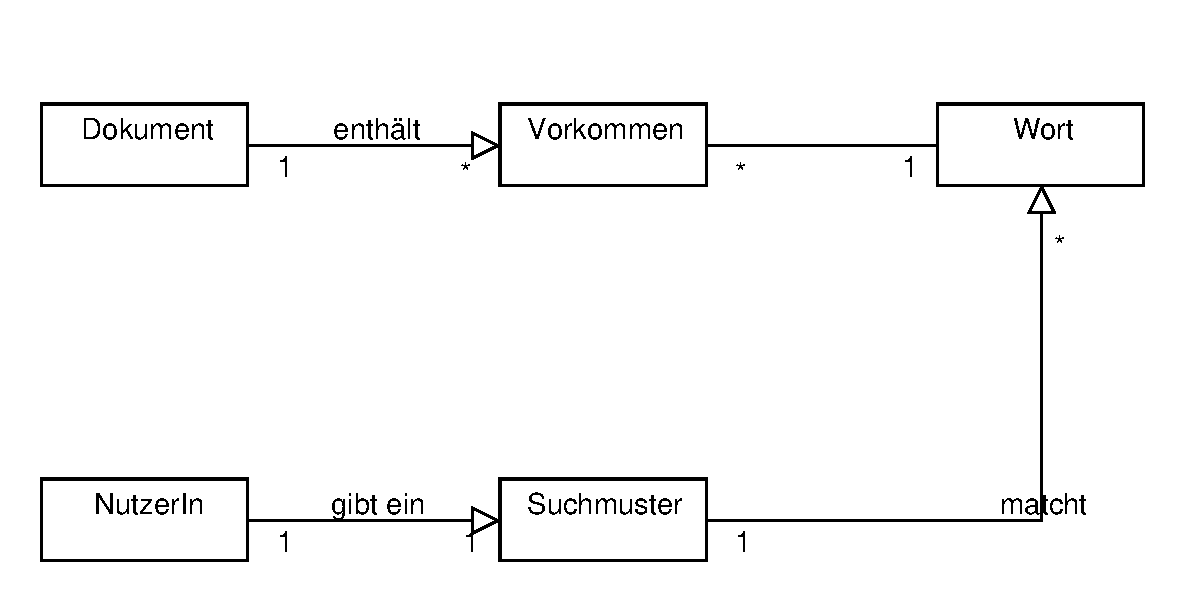
\includegraphics[scale=1]{resources/domain-model.pdf}
\end{textblock}
\newpage

\section{Architekturkonzept}
\label{uml-architecture}

\begin{textblock}{3}(3,3)
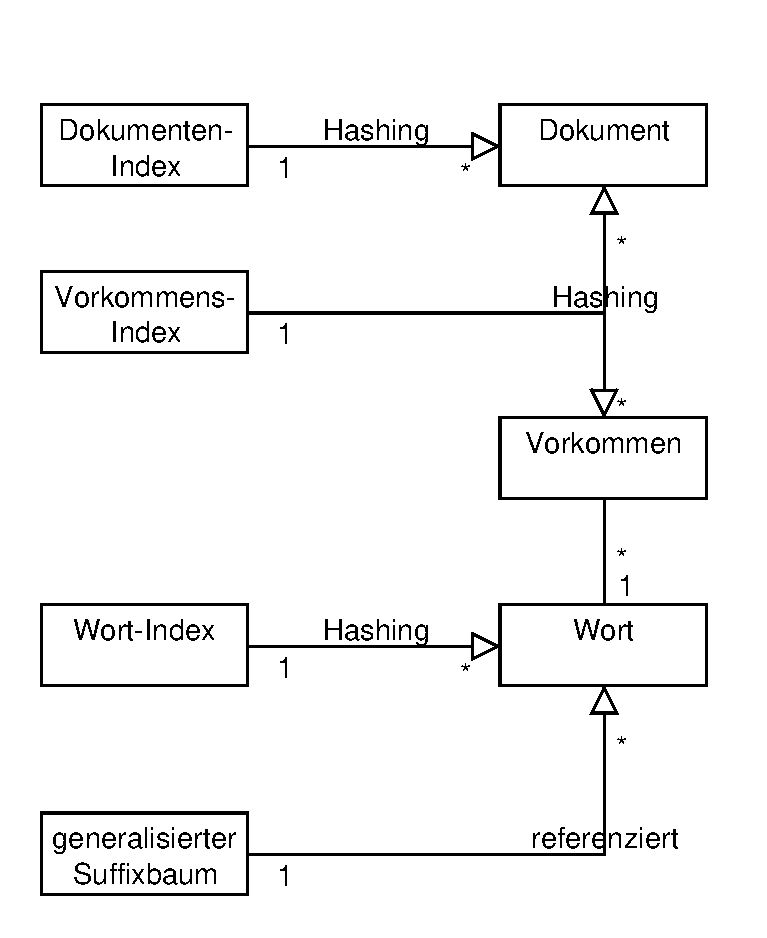
\includegraphics[scale=1]{resources/architecture.pdf}
\end{textblock}
\newpage

\section{Paketdiagramm}
\label{uml-package}

\begin{textblock}{3}(0.5,4)
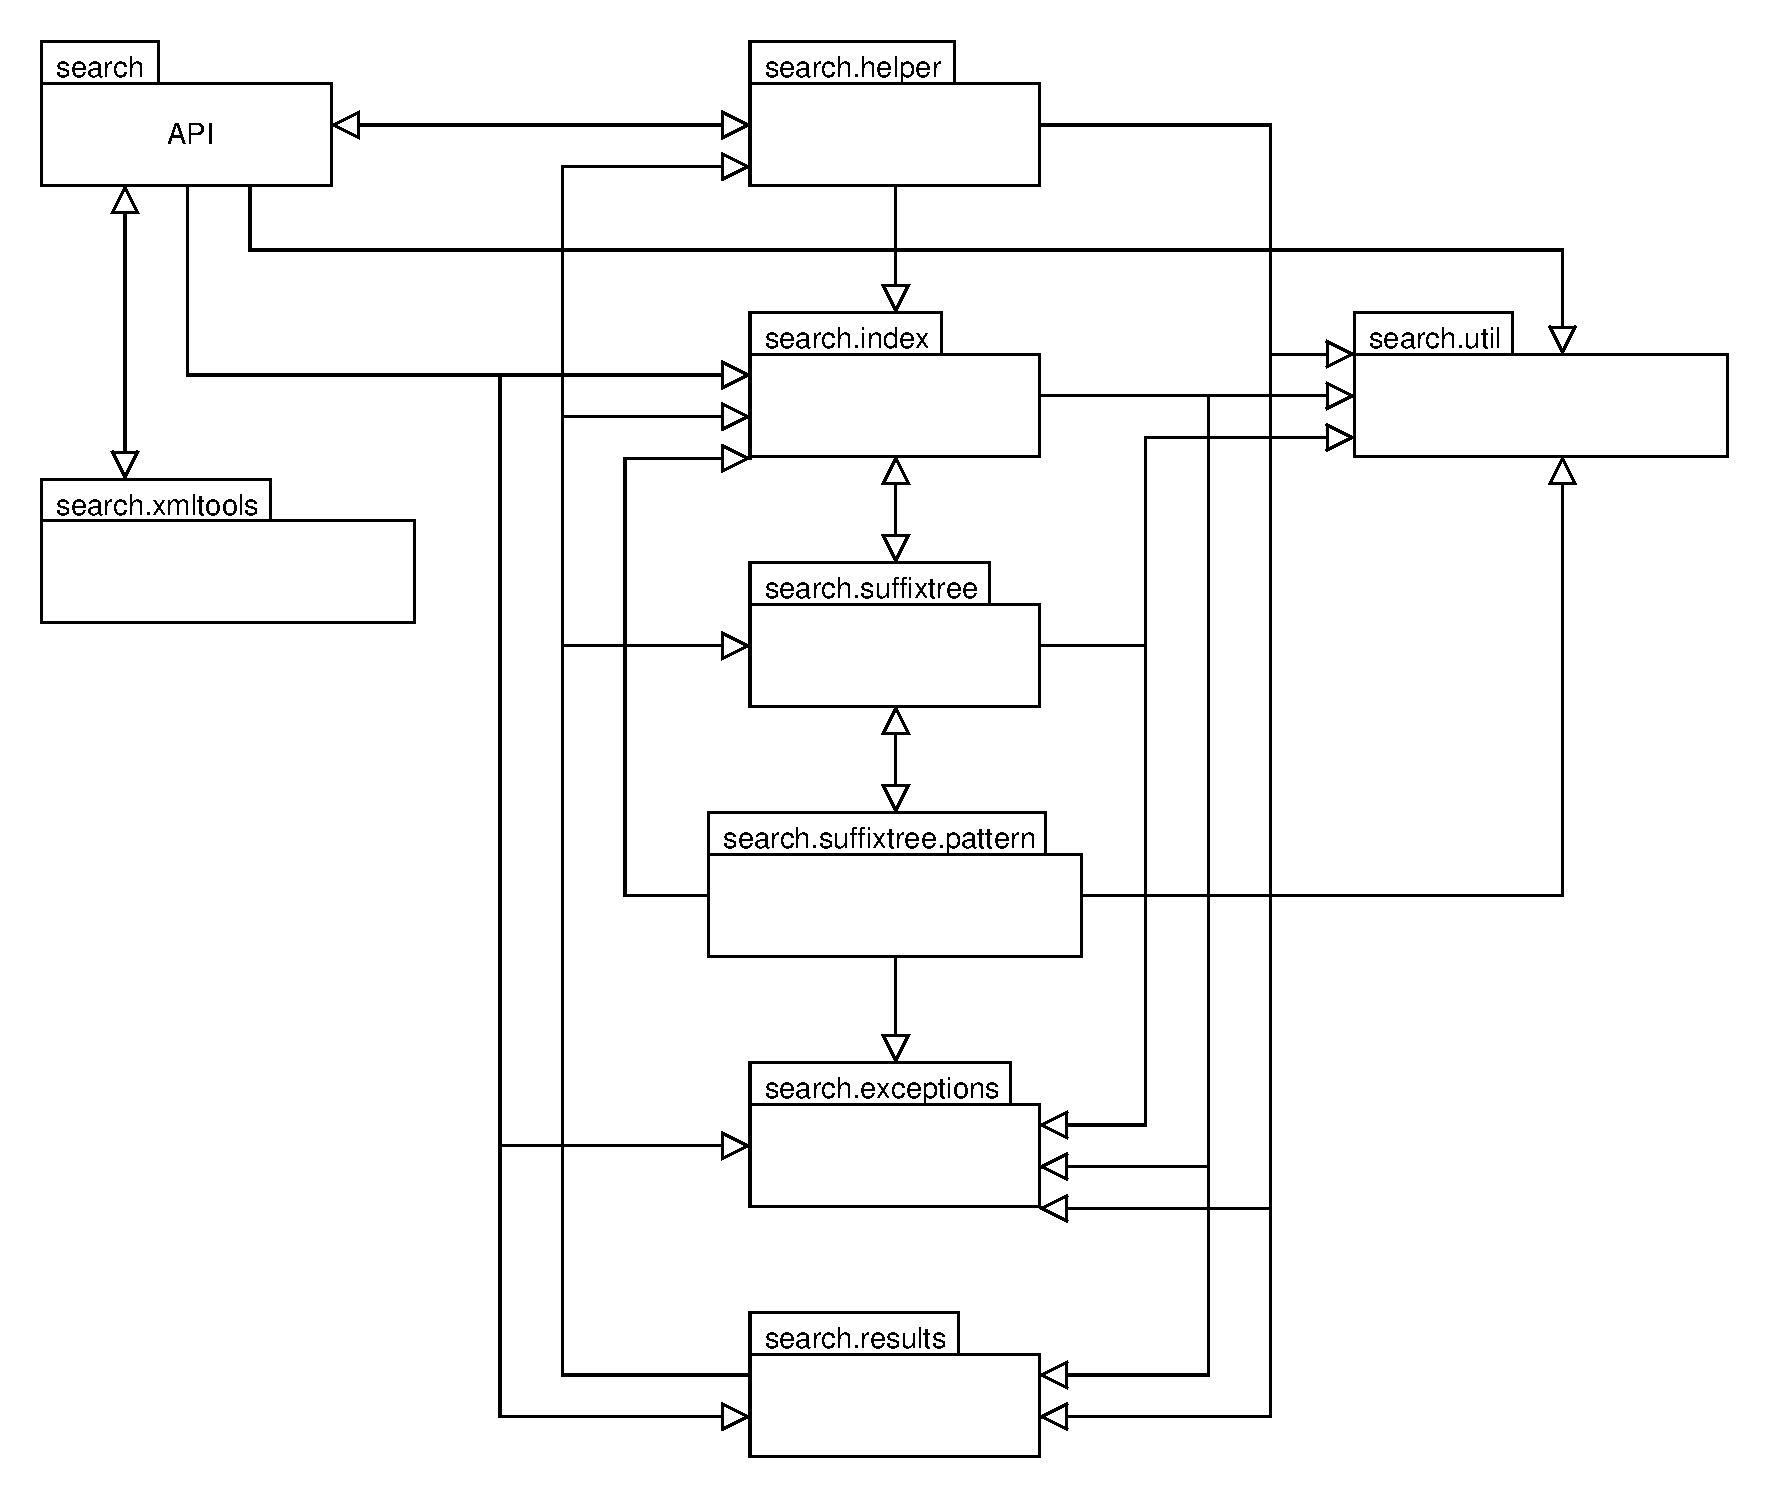
\includegraphics[scale=0.68]{resources/packages.pdf}
\end{textblock}

\newpage

\section{Klassendiagramm}
\label{uml-classes}

\begin{textblock}{3}(0.5,2.5)
\includegraphics[angle=270,scale=0.5]{resources/classes.pdf}
\end{textblock}

\newpage


\chapter{Konfiguration für Netbeans\texttrademark Profiling}
\label{profiling}

\paragraph{} Die Testkonfiguration für die Anwendung von NetBeans\texttrademark Profiling ist in der Klasse \texttt{ProfilingTestClass} im Hauptpaket der Anwendung abgelegt. Die Testdateien sind nicht beigelegt. Getestet wurde mit einer willkürlichen Auswahl deutscher und englischer Dateien (vornehmlich PDF-Dateien) mit möglichst vielen Worten (siehe auch \ref{fazit-complexity}). Für einen erneuten Test kann ein eigener Textdatensatz in den Ordner \texttt{test/data/mixed} im Netbeans-Arbeitsverzeichnis abgelegt werden.
\paragraph{} In NetBeans\texttrademark selbst müssen folgende Schritte durchgeführt werden, um das Profiling nachzuvollziehen:
\begin{itemize}
 \item In \texttt{ProfilingTestClass} den Testmodus einstellen (der Variable \texttt{testMode} irgendeinen Wert des enums zuweisen)
 \item Bei RAM-Tests: Die Variable \texttt{RAMTESTOCCLIMIT} einstellen. Die Variable legt das Limit indizierter Vorkommen fest, bis zu dem das Programm neue Dokumente einlesen wird. Je nachdem, wie viel Text die letzte eingelesene Datei enthält kann die Anzahl der tatsächlich eingelesenen Vorkommen deutlich darüber liegen. Sie liegt aber in jedem Falle nicht darunter.
 \item Den Netbeans\texttrademark Profiler kalibrieren.
 \item Den Netbeans\texttrademark Profiler für das Projekt entweder im Modus CPU oder Memory starten.
\end{itemize}
\paragraph{} Für diese Arbeit wurde NetBeans\texttrademark 7.2. benutzt und folgende Konfiguration verwendet:
\paragraph{CPU:} Quick (sampled); profile only project classes; keine profiling points.
\paragraph{Memory:} Record both object creation and garbage collection; track every 100 object allocations; keine profiling points.
\paragraph{} Das Profiling wurde auf einem CeBiTec-Rechner (nemo) durchgeführt, um eine möglichst praxisnahe Systemkonfiguration zu gewährleisten.



\chapter{Ukkonens Algorithmus}
\label{ukkonen}

\paragraph{} Eine ausführliche Beschreibung von Ukkonens Algorithmus mit Beweisen der linearen Laufzeit und des linearen Speicherverbrauchs ist bei Ukkonen selbst (siehe \cite{ukkonen}) oder bei Gusfield zu finden (siehe \cite{gusfield}). Hier ist lediglich die vorliegende Implementierung des Algorithmus für einen generalisierten Suffixbaum umrissen. Die Details dieser Implementierung können im Programmcode eingesehen werden.

\section{Definitionen}

\paragraph{} Für die weiteren Ausführung gelten die folgenden Definitionen:

\paragraph{Suffixbaum:} Ein Suffixbaum ist hier erst einmal nur als Baum, also als gerichteter Graph mit Wurzelknoten zu verstehen. Die Besonderheit des Suffixbaums ergibt sich aus den folgenden Definitionen.

\paragraph{Kante:} Eine Kante ist eine Kante im Suffixbaum. Sie enthält eine Referenz auf ein Wort, das im Suffixbaum enthalten ist sowie den Startindex (von 0 gezählt) und den Endindex (von 1 gezählt) des Teilwortes, das auf der Kante steht.

\paragraph{Interner Knoten:} Ein interner Knoten ist ein Knoten im Suffixbaum, von dem aus Kanten zu Blättern oder anderen internen Knoten verlaufen. Die Kanten werden über das erste Zeichen ihres Inhalts referenziert.

\paragraph{Pfad:} Ein Pfad zu einem Knoten ist die Konkatenation aller Zeichenketten auf Kanten, die vom Wurzelknoten zum Knoten führen.

\paragraph{Blatt:} Ein Blatt ist ein Knoten im Suffixbaum, von dem keine Kanten mehr ausgehen. Ein Blatt enthält eine Menge von Wort-IDs, für deren zugehörige Worte gilt: Der Pfad zum Blatt ist ein Suffix dieses Wortes.

\paragraph{active\_node (Variable):} Der momentan aktive, interne Knoten im Algorithmus.

\paragraph{active\_edge (Variable):} Das erste Zeichen des Inhalts der aktiven Kante, ausgehend vom \texttt{active\_node}.

\paragraph{active\_length (Variable):} Index (von 1 an gezählt) des momentan aktiven Zeichens auf der aktiven Kante.

\paragraph{currentChar (Variable):} Das momentan betrachtete Zeichen des neu einzufügenden Wortes.

\paragraph{remainder (Variable):} Anzahl der Zeichen, die vorgemerkt sind und noch in den Baum eingefügt werden müssen.

\paragraph{endPtr (Variable):} Referenz auf den Index des momentanen Zeichens \\(\texttt{currentChar}) des neuen Wortes (gezählt von 1).

\paragraph{suffixNode (Variable):} Der letzte, bei einer split-Operation (siehe \ref{ukkonen-splits}) behandelte Knoten. Das ist relevant für die Erzeugung von Suffix-Links.

\section{Initialisierung der Variablen und Benennung im Pseudocode}

\paragraph{} Die Variablen werden wie folgt initialisiert und in den folgenden Pseudocode-Abschnitten benannt:
\paragraph{}
\begin{tabularx}{\textwidth}{llX}
\hline
\textbf{Variable} & \textbf{Pseudocode-Name} & \textbf{Wert} \\ [0.1cm]
\hline
active\_node & $n_a$ & Wurzelknoten \\ [0.1cm]
\hline
active\_edge & $e_a$ & nicht gesetzt \\ [0.1cm]
\hline
active\_length & $l_a$ & 0 \\ [0.1cm]
\hline
currentChar & $c$ & erster Buchstabe des neuen Wortes \\ [0.1cm]
\hline
remainder & $r$ & 0 \\ [0.1cm]
\hline
endPtr & $e$ & 1 \\ [0.1cm]
\hline
suffixNode & $s$ & nicht gesetzt \\ [0.1cm]
\hline
\end{tabularx}

\newpage

\section{Allgemeines Vorgehen}

\paragraph{} Im Allgemeinen wird in Pseudocode-Algorithmus \ref{code-ukkonen-main} beschrieben vorgegangen.

\begin{algorithm}[H]
\caption{Allgemeines Vorgehen in Ukkonens Algorithmus (Methode \texttt{constructTree} in der Klasse \texttt{search.suffixtree.SuffixTreeConstructor})}
\label{code-ukkonen-main}
\begin{algorithmic}
\STATE{Sei $id$ die ID des neuen Wortes.}
\FORALL{Zeichen $c$ des neuen Wortes}
	\STATE{Inkrementiere den Wert von $e$.}
	\IF{Wurzelknoten hat noch keine Kante, die mit $c$ beginnt}
		\STATE{Erzeuge eine neue Kante mit einer Referenz auf $id$, dem Index von $c$ (gezählt von 0) und $e$.}
		\STATE{Füge die Kante an der Wurzel ein.}
		\STATE{Erzeuge ein neues Blatt am Ende der neuen Kante.}
		\STATE{Füge $id$ an das Blatt an.}
		\IF{$r$ $>$ $0$}
			\STATE{siehe \ref{ukkonen-splits}.}
		\ENDIF
	\ELSE
		\STATE{siehe \ref{ukkonen-existing}.}
	\ENDIF
	\STATE{Setze $s$ zurück.}
\ENDFOR
\STATE{siehe \ref{ukkonen-suffizes}.}
\end{algorithmic}
\end{algorithm}

\section{Bereits existierende Zeichen}
\label{ukkonen-existing}

\paragraph{} Wenn bereits existierende Zeichen auftreten wird vorgegangen wie in Pseudocode-Algorithmus \ref{code-ukkonen-existing} beschrieben. Es wird zuerst geprüft, ob ein Pfad für das neue Zeichen von der momentanen Baumposition aus existiert. Falls nicht, muss dieser Pfad geschaffen werden. Falls doch wird das aktuell eingelesene Zeichen vermerkt und der Algorithmus fährt fort.

\begin{algorithm}[H]
\caption{Behandlung bereits existierender Zeichen in Ukkonens Algorithmus (Methode \texttt{handleExistingChar} in der Klasse \texttt{search.suffixtree.SuffixTreeConstructor})}
\label{code-ukkonen-existing}
\begin{algorithmic}
\STATE{Sei $c$ das momentan betrachtete Zeichen des neuen Wortes.}
\IF{$l_a$ $\neq$ $0$}
	\STATE{Sei $k$ die Kante mit dem Anfangsbuchstaben $e_a$, die am Knoten $n_a$ startet.}
	\STATE{Sei ferner $c'$ das Zeichen, das (von 0 gezählt) im Teilwort, das auf $k$ steht, den Index $l_a$ hat, also das \underline{nächste} Zeichen im Baum nach dem eigentlich referenzierten, aktiven Zeichen.}
	\IF{$c$ $\neq$ $c'$}
		\STATE{siehe \ref{ukkonen-splits}.}
	\ENDIF
\ELSE
	\IF{$n_a$ besitzt \underline{keine} ausgehende Kante, die mit dem Zeichen $c$ beginnt}
		\STATE{siehe \ref{ukkonen-splits}.}
	\ENDIF
\ENDIF
\STATE{Inkrementiere $r$.}
\STATE{Inkrementiere $l_a$.}
\IF{$l_a$ $\neq$ $0$ und $e_a$ ist nicht gesetzt}
	\STATE{$e_a$ $=$ $c$.}
\ENDIF
\STATE{siehe \ref{ukkonen-jumps}.}
\end{algorithmic}
\end{algorithm}

\section{Splits}
\label{ukkonen-splits}

\paragraph{} Ein Split bedeutet, dass eine existierende Kante des Suffixbaumes irgendwo in der Mitte aufgespalten wird. Es wird an der Schnittstelle ein neuer Knoten eingefügt, vom dem zwei Kanten ausgehen. Eine zeigt auf den alten Zielknoten, eine auf einen neuen. In Ukkonens Algorithmus sind diese Zielknoten stets Blätter. Im Detail ist das Verfahren im Pseudocode-Algorithmus \ref{code-ukkonen-splits} beschrieben.

\begin{algorithm}[H]
\caption{Splits in Ukkonens Algorithmus (Methode \texttt{checkForSplits} in der Klasse \texttt{search.suffixtree.SuffixTreeConstructor})}
\label{code-ukkonen-splits}
\begin{algorithmic}
\STATE{Sei $id$ die ID des neuen Wortes.}
\WHILE{$r > 0$}
	\IF{$e_a$ ist gesetzt}
		\STATE{Sei $k$ die Kante, die von $n_a$ ausgeht und mit dem Zeichen $e_a$ beginnt.}
		\STATE{Sei $n_{alt}$ der Zielknoten von $k$.}
		\STATE{Erzeuge einen neuen internen Knoten $n_{split}$.}
		\IF{$s$ ist gesetzt}
			\STATE{Erzeuge einen Suffix-Link von $s$ zu $n_{split}$.}
		\ENDIF
		\STATE{setze $s$ $=$ $n_{split}$.}
		\STATE{Erzeuge eine neue Kante mit einer Referenz auf die Wort-ID, auf die $k$ referenziert, dem Startindex von $k$ $+$ $l_a$ und dem Endindex von $k$. Die Kante verläuft zwischen $n_{split}$ und $n_{alt}$.}
		\STATE{Erzeuge eine neue Kante mit einer Referenz auf $id$, dem Index von $c$ (gezählt von 0) und $e$.}
		\STATE{Füge die Kante an $n_{split}$ ein.}
		\STATE{Erzeuge ein neues Blatt am Ende der neuen Kante.}
		\STATE{Füge $id$ an das Blatt an.}
		\STATE{Setze den Endindex von $k$ auf den alten Startindex $+$ $l_a$.}
		\STATE{Setze den Zielknoten von $k$ auf $n_{split}$.}
		\STATE{siehe \ref{ukkonen-correct}.}
	\ELSE
		\IF{$n_a$ verfügt über eine Kante, die mit $c$ beginnt}
			\IF{$s$ ist gesetzt}
				\STATE{Erzeuge einen Suffix-Link von $s$ zu $n_a$.}
			\ENDIF
			\STATE{setze $s$ $=$ $n_a$.}
			\STATE{Beende die while-Schleife.}
		\ELSE
			\STATE{Erzeuge eine neue Kante mit einer Referenz auf $id$, dem Index von $c$ (gezählt von 0) und $e$.}
			\STATE{Füge die Kante an $n_a$ ein.}
			\STATE{Erzeuge ein neues Blatt am Ende der neuen Kante.}
			\STATE{Füge $id$ an das Blatt an.}
			\IF{$s$ ist gesetzt}
				\STATE{Erzeuge einen Suffix-Link von $s$ zu $n_a$.}
			\ENDIF
			\STATE{setze $s$ $=$ $n_a$.}
			\STATE{siehe \ref{ukkonen-correct}.}
		\ENDIF
	\ENDIF
\ENDWHILE
\end{algorithmic}
\end{algorithm}

\section{Korrektur der Baumposition}
\label{ukkonen-correct}

\paragraph{} Immer nach einer split-Operation und auch beim Einfügen von Worten, die ein Suffix bereits eingefügter Worte sind (siehe \ref{ukkonen-suffizes}) muss die Baumposition korrigiert werden. Dabei werden Suffix-Links ausgenutzt. Wie die Baumposition konkret korrigiert wird ist in Pseudocode-Algorithmus \ref{code-ukkonen-correct} nachzulesen.

\begin{algorithm}[H]
\caption{Korrektur der Baumposition in Ukkonens Algorithmus (Methode \texttt{correctActivePoint} in der Klasse \texttt{search.suffixtree.SuffixTreeConstructor})}
\label{code-ukkonen-correct}
\begin{algorithmic}
\STATE{Dekrementiere $r$.}
\IF{$n_a$ ist die Wurzel des Baumes}
	\STATE{Dekrementiere $l_a$.}
	\IF{$l_a$ ist auf $0$ gesunken}
		\STATE{Setze $e_a$ zurück.}
	\ELSE
		\STATE{Setze $e_a$ auf das vorherige Zeichen im neuen Wort.}
	\ENDIF
\ELSE
	\IF{$n_a$ hat einen Suffix-Link}
		\STATE{Setze $n_a$ auf den Suffix-Link von $n_a$.}
	\ELSE
		\STATE{Setze $n_a$ auf die Wurzel des Baumes.}
	\ENDIF
\ENDIF
\STATE{siehe \ref{ukkonen-jumps}.}
\end{algorithmic}
\end{algorithm}

\section{Sprünge}
\label{ukkonen-jumps}

\paragraph{} Sprünge werden immer dann ausgeführt, wenn die Länge der momentan aktiven Kante kürzer oder gleich \texttt{active\_length} ist. Ein Sprung bedeutet, dass \texttt{active\_node} auf den Zielknoten der aktiven Kante gesetzt, \texttt{active\_length} um die Länge der momentan aktiven Kante verkürzt und schließlich die aktive Kante neu gesetzt wird. Die Details dieses Prozesses sind im Pseudocode-Algorithmus \ref{code-ukkonen-jump} beschrieben.

\begin{algorithm}[H]
\caption{Sprünge in Ukkonens Algorithmus (Methode \texttt{checkForJumps} in der Klasse \texttt{search.suffixtree.SuffixTreeConstructor})}
\label{code-ukkonen-jump}
\begin{algorithmic}
\IF{$e_a$ ist gesetzt}
	\STATE{Sei $k$ die Kante, die mit $e_a$ beginnt und an $n_a$ startet.}
	\STATE{Sei $l_a'$ die Länge des Inhaltes von $k$.}
	\WHILE{$l_a'$ $\le$ $l_a$}
		\STATE{Setze $n_a$ auf den Zielknoten von $k$.}
		\STATE{Setze $l_a$ $=$ $l_a-l_a'$.}
		\IF{$l_a$ ist auf $0$ abgesunken}
			\STATE{Setze $e_a$ zurück.}
			\STATE{Setze $l_a'$ $=$ $1$.}
		\ELSE
			\STATE{Setze $e_a$ auf den Buchstaben des neuen Wortes, der $l_a'$ Zeichen weiter liegt.}
			\STATE{Sei $k$ die Kante, die mit $e_a$ beginnt und an $n_a$ startet.}
			\STATE{Setze $l_a'$ auf die Länge von $k$.}
		\ENDIF
	\ENDWHILE
\ENDIF
\end{algorithmic}
\end{algorithm}

\section{Suffixe bereits eingetragener Worte}
\label{ukkonen-suffizes}

\paragraph{} Dass ein neues Wort ein Suffix eines bereits eingefügten Wortes ist kann daran erkannt werden, dass der \texttt{remainder} auch nach Durchlauf von Ukkonens Algorithmus noch größer 0 ist\footnote{genau genommen größer 1, weil ein Endzeichen mit betrachtet werden muss. Dieses Detail wird hier aber nicht weiter behandelt.}. Das bedeutet: Alle Suffixe dieses neuen Wortes sind bereits im Baum. Das kann aber nur sein, wenn entweder das Wort selbst bereits in den Baum eingefügt wurde oder aber ein Wort, dessen echtes Suffix das neue Wort ist. In diesem Fall zeigt die momentane Position im Baum nach Durchlauf des Algorithmus die Position des Blattes an, dessen Pfad das gesamte neue Wort ist. Es muss also nur an diesem Blatt die ID des neuen Wortes eingetragen und dann zu allen Suffixen des momentanen Pfades gesprungen werden. Das ist durch Suffix-Links einfach zu lösen und geschieht nach wie vor in linearer Zeit. Das genaue Vorgehen kann in Pseudocode-Algorithmus \ref{code-ukkonen-suffizes} nachgelesen werden.

\begin{algorithm}[H]
\caption{Behandlung des Falles, dass ein neues Wort ein Suffix eines bereits eingefügten Wortes ist (Zweiter Teil der Methode \texttt{constructTree} in der Klasse \texttt{search.suffixtree.SuffixTreeConstructor})}
\label{code-ukkonen-suffizes}
\begin{algorithmic}
\STATE{Sei $id$ die ID des neuen Wortes.}
\WHILE{$r$ $>$ $0$}
	\STATE{Sei $k$ die Kante, die mit $e_a$ beginnt und an $n_a$ startet.}
	\STATE{Dann ist der Zielknoten $n_k$ von $k$ dank Ukkonens Algorithmus garantiert ein Blatt.}
	\STATE{Trage $id$ an $n_k$ ein.}
	\STATE{Siehe \ref{ukkonen-correct}.}
\ENDWHILE
\end{algorithmic}
\end{algorithm}

\end{appendix}
\end{document}